\documentclass[a4paper]{article}

\def\npart {III}
\def\nterm {Easter}
\def\nyear {2017}
\def\nlecturer {N.\ S.\ Manton and D.\ Stuart}
\def\ncourse {Classical and Quantum Solitons}
\def\nisofficial {}

\input{header}

\usepackage[compat=1.1.0]{tikz-feynman}
\tikzfeynmanset{/tikzfeynman/momentum/arrow shorten = 0.3}
\tikzfeynmanset{/tikzfeynman/warn luatex = false}

\begin{document}
\maketitle
{\small
\setlength{\parindent}{0em}
\setlength{\parskip}{1em}
Solitons are solutions of classical field equations with particle-like properties. They are localised in space, have finite energy and are stable against decay into radiation. The stability usually has a topological explanation. After quantisation, they give rise to new particle states in the underlying quantum field theory that are not seen in perturbation theory. We will focus mainly on kink solitons in one space dimension, on gauge theory vortices in two dimensions, and on Skyrmions in three dimensions.

\subsubsection*{Pre-requisites}
This course assumes you have taken Quantum Field Theory and Symmetries, Fields and Particles. The small amount of topology that is needed will be developed during the course.
\subsubsection*{Reference}
N.\ Manton and P.\ Sutcliffe, \emph{Topological Solitons}, CUP, 2004
}
\tableofcontents

\setcounter{section}{-1}
\section{Introduction}
Given a classical field theory, if we want to ``quantize'' it, then we find the vacuum of the theory, and then do perturbation theory around this vacuum. If there are multiple vacua, then what we did was that we arbitrarily picked a vacuum, and then expanded around that vacuum.

However, these field theories with multiple vacua often contain \emph{soliton} solutions. These are localized, smooth solutions of the classical field equations, and they ``connect multiple vacuums''. To quantize these solitons solutions, we fix such a soliton, and use it as the ``background''. We then do perturbation theory around these solutions, but this is rather tricky to do. Thus, in a lot of the course, we will just look at the classical part of the theory.

Recall that when quantizing our field theories in perturbation theory, we obtain particles in the quantum theory, despite the classical theory being completely about fields. It turns out solitons also behave like particles, and they are a \emph{new} type of particles. These are non-perturbative phenomena. If we want to do the quantum field theory properly, we have to include these solitons in the quantum field theory. In general this is hard, and so we are not going to develop this a lot.

What does it mean to say that solitons are like particles? In relativistic field theories, we find these solitons have a classical energy. We define the ``mass'' $M$ of the soliton to be the energy in the ``rest frame''. Since this is relativistic, we can do a Lorentz boost, and we obtain a moving soliton. Then we obtain an energy-momentum relation of the form
\[
  E^2 - \mathbf{P} \cdot \mathbf{P} = M^2.
\]
This is a Lorentz-invariant property of the soliton. Together with the fact that the soliton is localized, this is a justification for thinking of them as particles.

These particles differ from the particles of perturbative quantum fields, as they have rather different properties. Interesting solitons have a \emph{topological} character different from the classical vacuum. Thus, at least naively, they cannot be thought of perturbatively.

There are also non-relativistic solitons, but they usually don't have interpretations as particles. These appear, for example, as defects in solids. We will not be interested in these much.

What kinds of theories have solitons? To obtain solitons, we definitely need a non-linear field structure and/or non-linear equations. Thus, free field theories with quadratic Lagrangians such as Maxwell theory do not have solitons. We need interaction terms.

Note that in QFT, we dealt with interactions using the interaction picture. We split the Hamiltonian into a ``free field'' part, which we solve exactly, and the ``interaction'' part. However, to quantize solitons, we need to solve the full interacting field equations \emph{exactly}.

Having interactions is not enough for solitons to appear. To obtain solitons, we also need some non-trivial vacuum topology. In other words, we need more than one vacuum. This usually comes from symmetry breaking, and often gauge symmetries are involved.

In this course, we will focus on three types of solitons.
\begin{itemize}
  \item In one (space) dimension, we have kinks. We will spend $4$ lectures on this.

  \item In two dimensions, we have vortices. We will spend $6$ lectures on this.

  \item In three dimensions, there are monopoles and Skyrmions. We will only study Skyrmions, and will spend $6$ lectures on these.
\end{itemize}
These examples are all relativistic. Non-relativistic solitons include \emph{domain walls}, which occur in ferromagnets, and two-dimensional ``baby'' Skyrmions, which are seen in exotic magnets, but we will not study these.

In general, solitons appear in all sorts of different actual, physical scenarios such as in condensed matter physics, optical fibers, superconductors and exotic magnets. ``Cosmic strings'' have also been studied. Since we are mathematicians, we probably will not put much focus on these actual applications. However, we can talk a bit more about Skyrmions.

Skyrmions are solitons in an \emph{effective field theory} of interacting pions, which are thought to be the most important hadrons because they are the lightest. This happens in spite of the lack of a gauge symmetry. While pions have no baryon number, the associated solitons have a topological charge identified with baryon number. This baryon number is conserved for topological reasons.

Note that in QCD, baryon number is conserved because the quark number is conserved. Experiments tried extremely hard to find proton decay, which would be a process that involves baryon number change, but we cannot find such examples. We have very high experimental certainty that baryon number is conserved. And if baryon number is topological, then this is a very good reason for the conservation of baryon number.

Skyrmions give a model of low-energy interactions of baryons. This leads to an (approximate) theory of nucleons (proton and neutron) and larger nuclei, which are bound states of any number of protons and neutrons.

For these ideas to work out well, we need to eventually do quantization. For example, Skyrmions by themselves do not have spin. We need to quantize the theory before spins come out. Also, Skyrmions cannot distinguish between protons and neutrons. These differences only come up after we quantize.

\section{\tph{$\phi^4$}{phi4}{&straightphi;<sup>4</sup>} kinks}
\subsection{Kink solutions}
In this section, we are going to study \term{$\phi^4$ kinks}\index{kink}\index{kink!$\phi^4$}. These occur in $1 + 1$ dimensions, and involve a single scalar field $\phi(x, t)$. In higher dimensions, we often need many fields to obtain solitons, but in the case of 1 dimension, we can get away with a single field.

In general, the \term{Lagrangian density} of such a scalar field theory is of the form
\[
  \mathcal{L} = \frac{1}{2} \partial_\mu \phi \partial^\mu \phi - U(\phi)
\]
for some potential $U(\phi)$ polynomial in $\phi$. Note that in $1 + 1$ dimensions, any such theory is renormalizable. Here we will choose the Minkowski metric to be
\[
  \eta^{\mu\nu} =
  \begin{pmatrix}
    1 & 0\\
    0 & -1
  \end{pmatrix},
\]
with $\mu, \nu = 0, 1$. Then the \term{Lagrangian} is given by
\[
  L = \int_{-\infty}^\infty \mathcal{L}\;\d x = \int_{-\infty}^\infty \left(\frac{1}{2} \partial_\mu \phi \partial^\mu \phi - U(\phi)\right)\;\d x,
\]
and the \term{action} is
\[
  S[\phi] = \int L\;\d t = \int \mathcal{L} \;\d x\;\d t.
\]

There is a non-linearity in the field equations due to a potential $U(\phi)$ with \emph{multiple vacua}. We need multiple vacua to obtain a soliton. The kink stability comes from the \emph{topology}. It is very simple here, and just comes from counting the discrete, distinct vacua.

As usual, we will write
\[
  \dot{\phi} = \frac{\partial \phi}{\partial t},\quad \phi' = \frac{\partial \phi}{\partial x}.
\]
Often it is convenient to (non-relativistically) split the Lagrangian as
\[
  L = T - V,
\]
where
\[
  T = \int \frac{1}{2} \dot{\phi}^2\;\d x,\quad V = \int \left(\frac{1}{2} \phi'^2 + U(\phi)\right)\;\d x.
\]
In higher dimensions, we separate out $\partial_\mu \phi$ into $\dot{\phi}$ and $\nabla \phi$.

The classical field equation comes from the condition that $S[\phi]$ is stationary under variations of $\phi$. By a standard manipulation, the field equation turns out to be
\[
  \partial_\mu \partial^\mu \phi + \frac{\d U}{\d \phi} = 0.
\]
This is an example of a Klein--Gordon type of field equation, but is non-linear if $U$ is not quadratic. It is known as the \emph{non-linear Klein--Gordon equation}\index{Klein--Gordon equation!non-linear}.

We are interested in a soliton that is a static solution. For a static field, the time derivatives can be dropped, and this equation becomes
\[
  \frac{\d^2 \phi}{\partial x^2} = \frac{\d U}{\d \phi}.
\]
Of course, the important part is the choice of $U$! In $\phi^4$ theory, we choose
\[
  U(\phi) = \frac{1}{2} (1 - \phi^2)^2.
\]
This is mathematically the simplest version, because we set all coupling constants to $1$.

The importance of this $U$ is that it has two minima:
\begin{center}
  \begin{tikzpicture}
    \draw [->](-3, -1) -- (3, -1) node [right] {$\phi$};
    \draw [->] (0, -1.5) -- (0, 3) node [above] {$U(\phi)$};

    \draw [mblue, thick, domain=-2.4:2.4, samples=50] plot [smooth] (\x, {4 * ((\x/2)^4 - (\x/2)^2)});

    \node at (-1.414, -1) [below] {$-1$};
    \node at (1.414, -1) [below] {$1$};
  \end{tikzpicture}
\end{center}
The two classical vacua are
\[
  \phi(x) \equiv 1,\quad \phi(x) \equiv -1.
\]
This is, of course, not the only possible choice. We can, for example, include some parameters and set
\[
  U(\phi) = \lambda(m^2 - \phi^2)^2.
\]
If we are more adventurous, we can talk about a $\phi^6$ theory with
\[
  U(\phi) = \lambda \phi^2 (m^2 - \phi^2)^2.
\]
In this case, we have $3$ minima, instead of $2$. Even braver people can choose
\[
  U(\phi) = 1 - \cos \phi.
\]
This has \emph{infinitely} many minima. The field equation involves a $\sin \phi$ term, and hence this theory is called the \term{sine-Gordon theory} (a pun on the name Klein--Gordon, of course).

The sine-Gordon theory is a special case. While it seems like the most complicated potential so far, it is actually \emph{integrable}\index{integrability}. This implies we can find explicit exact solutions involving multiple, interacting solitons in a rather easy way. However, integrable systems is a topic for another course, namely IID Integrable Systems.

For now, we will focus on our simplistic $\phi^4$ theory. As mentioned, there are two vacuum field configurations, both of zero energy. We will in general use the term ``\term{field configuration}'' to refer to fields at a given time that are not necessarily solutions to the classical field equation, but in this case, the vacua are indeed solutions.

If we wanted to quantize this $\phi^4$ theory, then we have to pick one of the vacua and do perturbation theory around it. This is known as \term{spontaneous symmetry breaking}. Of course, by symmetry, we obtain the same quantum theory regardless of which vacuum we expand around.

However, as we mentioned, when we want to study solitons, we have to involve \emph{both} vacua. We want to consider solutions that ``connect'' these two vacua. In other words, we are looking for solutions that look like
\begin{center}
  \begin{tikzpicture}
    \draw [->] (-3, 0) -- (3, 0) node [right] {$x$};
    \draw [->] (0, -2) -- (0, 2) node [above] {$\phi$};

    \draw [mblue, thick, domain=-3:3] plot [smooth] (\x, {tanh(1.5*(\x + 1))});

    \draw [dashed] (-3, 1) -- (3, 1);
    \draw [dashed] (-3, -1) -- (3, -1);

    \node [circ] at (-1, 0) {};
    \node [anchor = north west] at (-1, 0) {$a$};
  \end{tikzpicture}
\end{center}
This is known as a \term{kink solution}.

To actually find such a solution, we need the full field equation, given by
\[
  \frac{\d^2 \phi}{\d x^2} = -2 (1 - \phi^2) \phi.
\]
Instead of solving this directly, we will find the kink solutions by considering the energy, since this method generalizes better.

We will work with a general potential $U$ with minimum value $0$. From Noether's theorem, we obtain a conserved energy
\[
  E = \int \left(\frac{1}{2} \dot{\phi}^2 + \frac{1}{2} \phi'^2 + U(\phi)\right)\;\d x.
\]
For a static field, we drop the $\dot{\phi}^2$ term. Then this is just the $V$ appearing in the Lagrangian. By definition, the field equation tells us the field is a stationary point of this energy. To find the kink solution, we will in fact find a \emph{minimum} of the energy.

Of course, the global minimum is attained when we have a vacuum field, in which case $E = 0$. However, this is the global minimum only if we don't impose any boundary conditions. In our case, the kinks satisfy the boundary conditions ``$\phi(\infty) = 1$'', ``$\phi(-\infty) = -1$'' (interpreted in terms of limits, of course). The kinks will minimize energy subject to these boundary conditions.

These boundary conditions are important, because they are ``topological''. Eventually, we will want to understand the dynamics of solitons, so we will want to consider fields that evolve with time. From physical considerations, for any fixed $t$, the field $\phi(x, t)$ must satisfy $\phi(x, t) \to \text{vacuum}$ as $x \to \pm \infty$, or else the field will have infinite energy. However, the vacuum of our potential $U$ is discrete. Thus, if $\phi$ is to evolve continuously with time, the boundary conditions must not evolve with time! At least, this is what we expect classically. Who knows what weird tunnelling can happen in quantum field theory.

So from now on, we fix some boundary conditions $\phi(\infty)$ and $\phi(-\infty)$, and focus on fields that satisfy these boundary conditions. The trick is to write the potential in the form
\[
  U (\phi) = \frac{1}{2} \left(\frac{\d W (\phi)}{\d \phi}\right)^2.
\]
If $U$ is non-negative, then we can always find $W$ in principle --- we take the square root and then integrate it. However, in practice, this is useful only if we can find a simple form for $W$. Let's assume we've done that. Then we can write
\begin{align*}
  E &= \frac{1}{2} \int \left(\phi'^2 + \left(\frac{\d W}{\d \phi}\right)^2 \right)\;\d x\\
  &= \frac{1}{2} \int \left(\phi' \mp \frac{\d W}{\d \phi}\right)^2\;\d x \pm \int \frac{\d W}{\d \phi} \frac{\d \phi}{\d x} \;\d x\\
  &= \frac{1}{2} \int \left(\phi' \mp \frac{\d W}{\d \phi}\right)^2\;\d x \pm \int \d W\\
  &= \frac{1}{2} \int \left(\phi' \mp \frac{\d W}{\d \phi}\right)^2\;\d x \pm (W(\phi(\infty)) - W(\phi(-\infty))).
\end{align*}
The second term depends purely on the boundary conditions, which we have fixed. Thus, we can minimize energy if we can make the first term vanish! Note that when completing the square, the choice of the signs is arbitrary. However, if we want to set the first term to be $0$, the second term had better be non-negative, since the energy itself is non-negative! Hence, we will pick the sign such that the second term is $\geq 0$, and then the energy is minimized when
\[
  \phi' = \pm \frac{\d W}{\d \phi}.
\]
In this case, we have
\[
  E = \pm (W(\infty) - W(-\infty)).
\]
These are known as the \term{Bogomolny equation} and the \term{Bogomolny energy bound}. Note that if we picked the other sign, then we cannot solve the differential equation $\phi' = \pm \frac{\d W}{\d \phi}$, because we know the energy must be non-negative.

For the $\phi^4$ kink, we have
\[
  \frac{\d W}{\d \phi} = 1 - \phi^2.
\]
So we pick
\[
  W = \phi - \frac{1}{3} \phi^3.
\]
So when $\phi = \pm 1$, we have $W = \pm \frac{2}{3}$. We need to choose the $+$ sign, and then we know the energy (and hence mass) of the kink is
\[
  E \equiv M = \frac{4}{3}.
\]
We now solve for $\phi$. The equation we have is
\[
  \phi' = 1 - \phi^2.
\]
Rearranging gives
\[
  \frac{1}{1 - \phi^2} \d \phi = \d x,
\]
which we can integrate to give
\[
  \phi (x) = \tanh (x - a).
\]
This $a$ is an arbitrary constant of integration, labelling the intersection of the graph of $\phi$ with the $x$-axis. We think of this as the ``\emph{location}'' of the kink.

Note that there is not a unique solution, which is not unexpected by translation invariance. Instead, the solutions are labeled by a parameter $a$. This is known as a \term{modulus} of the solution. In general, there can be multiple moduli, and the space of all possible values of the moduli of static solitons is known as the \term{moduli space}. In the case of a kink, the moduli space is just $\R$.

Is this solution stable? We obtained this kink solution by minimizing the energy within this topological class of solutions (i.e.\ among all solutions with the prescribed boundary conditions). Since a field cannot change the boundary conditions during evolution, it follows that the kink must be stable.

Are there other soliton solutions to the field equations? The solutions are determined by the boundary conditions. Thus, we can classify all soliton solutions by counting all possible combinations of the boundary conditions. We have, of course, two vacuum solutions $\phi \equiv 1$ and $\phi \equiv -1$. There is also an \term{anti-kink}\index{kink!anti-} solution obtained by inverting the kink:
\[
  \phi(x) = - \tanh (x - b).
\]
This also has energy $\frac{4}{3}$.

\subsection{Dynamic kink}
We now want to look at kinks that move. Given what we have done so far, this is trivial. Our theory is Lorentz invariant, so we simply apply a Lorentz boost. Then we obtain a field
\[
  \phi(x, t) = \tanh \gamma (x - vt),
\]
where, as usual
\[
  \gamma = (1 - v^2)^{-1/2}.
\]
But this isn't all. Notice that for small $v$, we can approximate the solution simply by
\[
  \phi(x, t) = \tanh (x - vt).
\]
This looks like a kink solution with a modulus that varies with time slowly. This is known as the \term{adiabatic} point of view.

More generally, let's consider a ``moving kink'' field
\[
  \phi(x, t) = \tanh (x - a(t))
\]
for some function $a(t)$. In general, this is not a solution to the field equation, but if $\dot{a}$ is small, then it is ``approximately a solution''.

We can now explicitly compute that
\[
  \dot{\phi} = - \frac{\d a}{\d t} \phi'.
\]
Let's consider fields of this type, and look at the Lagrangian of the field theory. The kinetic term is given by
\[
  T = \int \frac{1}{2} \dot{\phi}^2\;\d x = \frac{1}{2} \left(\frac{\d a}{\d t}\right)^2 \int \phi'^2 \;\d x = \frac{1}{2} M \left(\frac{\d a}{\d t}\right)^2.
\]
To derive this result, we had to perform the integral $\int \phi'^2 \;\d x$, and if we do that horrible integral, we will find a value that happens to be equal to $M = \frac{4}{3}$. Of course, this is not a coincidence. We can derive this result from Lorentz invariance to see that the result of integration is manifestly $M$.

The remaining part of the Lagrangian is less interesting. Since it does not involve taking time derivatives, the time variation of $a$ is not seen by it, and we simply have a constant
\[
  V = \frac{4}{3}.
\]
Then the original field Lagrangian becomes a particle Lagrangian
\[
  L = \frac{1}{2}M \dot{a}^2 - \frac{4}{3}.
\]

Note that when we first formulated the field theory, the action principle required us to find a field that extremizes the action \emph{among all fields}. However, what we are doing now is to restrict to the set of kink solutions only, and then when we solve the variational problem arising from this Lagrangian, we are extremizing the action among fields of the form $\tanh (x - a(t))$. We can think of this as motion in a ``valley'' in the field configuration space. In general, these solutions will not also extremize the action among all fields. However, as we said, it will do so ``approximately'' if $\dot{a}$ is small.

We can obtain an effective equation of motion
\[
  M \ddot{a} = 0,
\]
which is an equation of motion for the variable $a(t)$ \emph{in the moduli space}.

Of course, the solution is just given by
\[
  a(t) = vt + \mathrm{const},
\]
where $v$ is an arbitrary constant, which we interpret as the velocity. In this formulation, we do not have any restrictions on $v$, because we took the ``non-relativistic approximation''. This approximation breaks down when $v$ is large.

There is a geometric interpretation to this. We can view the equation of motion $M\ddot{a} = 0$ as the \emph{geodesic equation} in the moduli space $\R$, and we can think of the coefficient $M$ as specifying a Riemannian metric on the moduli space. In this case, the metric is (a scalar multiple of) the usual Euclidean metric $(\d a)^2$.

This seems like a complicated way of describing such a simple system, but this picture generalizes to higher-dimensional systems and allows us to analyze multi-soliton dynamics, in particular, the dynamics of vortices and monopoles.

%We can find the dynamics of $a(t)$ from the Lagrangian of the field theory. Thus, we are reducing the ``field dynamics'' to the ``particle dynamics''. We have
%\[
% T = \int \frac{1}{2} \dot{\phi}^2\;\d x = \frac{1}{2} \left(\frac{\d a}{\d t}\right)^2 \int \phi'^2 \;\d x = \frac{1}{2} M \left(\frac{\d a}{\d t}\right)^2.
%\]
%The factor of $M$ just comes from doing the (tricky) integral explicitly, but we can also work it out from more general principles to make it manifestly $M$, and this is known as Derrick's theorem.
%
%Thus, the kink behaves like a particle with mass $M$! How about the potential energy? The potential energy is \emph{not} time-dependent. We simply integrate some polynomial of $\phi$ over all $x$, and the shift by $a$ does not make a difference. In this case, we have
%\[
% V = \frac{4}{3}.
%\]
%So we've reduced the field Lagrangian to a particle Lagrangian
%\[
% L = \frac{1}{2}M \dot{a}^2 - \frac{4}{3}.
%\]
%We can think of this as motion in a \term{valley} in the field configuration space. We are drifting in the energy minima in the field configuration space.
%
%This method is powerful, and applies to multi-soliton dynamics in high dimensions. From this, we obtain an effective equation of motion in moduli space
%\[
% M \ddot{a} = 0.
%\]
%This has \emph{geometric} interpretation as geometric motion in the moduli space. The moduli space is just the real line $\R$ with its standard metric. We can think of the coefficient $M$ as a Riemannian metric, which happens to be constant (as a function of $a$) in this case.
%
%Of course, the solution is
%\[
% a(t) = vt + \mathrm{const},
%\]
%where $v$ is an arbitrary constant, namely velocity.
%
%In this approximation, $v$ can be anything, and the approximation does not see the speed of light. However, as we plug this back into the actual field equation, we see that the approximation breaks down when $v$ is large.
%
%This motion in moduli space is not exact, but is accurate in the non-relativistic approximation.
%
%This was all rather trivial in our case of kinks. However, it is also important and allows us to analyze the motion of several solitons in higher dimension.
%
%Note that here we started with a Lagrangian that is quadratic in time derivatives of the field. When we pass on to solitons, we have a term that is quadratic in the time derivative in the moduli, and the coefficients provide a Riemannian geometry on the moduli space.

We might ask ourselves if there are multi-kinks in our theory. There aren't in the $\phi^4$ theory, because we saw that the solutions are classified by the boundary conditions, and we have already enumerated all the possible boundary conditions. In more complicated theories like sine-Gordon theory, multiple kinks are possible.

However, while we cannot have two kinks in $\phi^4$ theory, we can have a kink followed by an anti-kink, or more of these pairs. This actually lies in the ``vacuum sector'' of the theory, but it still looks like it's made up of kinks and anti-kinks, and it is interesting to study these.

\subsection{Soliton interactions}
We now want to study interactions between kinks and anti-kinks, and see how they cause each other to move. So far, we were able to label the position of the particle by its ``center'' $a$, and thus we can sensibly talk about how this center moves. However, this center is well-defined only in the very special case of a pure kink or anti-kink, where we can use symmetry to identify the center. If there is some perturbation, or if we have a kink and an anti-kink, it is less clear what should be considered the center.

Fortunately, we can still talk about the momentum of the field, even if we don't have a well-defined center. Indeed, since our theory has translation invariance, Noether's theorem gives us a conserved charge which is interpreted as the momentum.

Recall that for a single scalar field in $1 + 1$ dimensions, the Lagrangian density can be written in the form
\[
  \mathcal{L} = \frac{1}{2} \partial_\mu \phi \partial^\mu \phi - U(\phi).
\]
Applying Noether's theorem, to the translation symmetry, we obtain the \term{energy-momentum tensor}
\[
  T^\mu_\nu = \frac{\partial \mathcal{L}}{\partial (\partial_\mu \phi)} \partial_\nu \phi - \delta^\mu_\nu \mathcal{L} = \partial^\mu \phi \partial_\nu \phi - \delta^\mu_\nu \mathcal{L}.
\]
Fixing a time and integrating over all space, we obtain the conserved energy and conserved momentum. These are
\begin{align*}
  E &= \int_{-\infty}^\infty T^0\!_0 \;\d x = \int_{-\infty}^\infty \left(\frac{1}{2}\dot{\phi}^2 + \frac{1}{2} \phi'^2 + U(\phi)\right)\;\d x,\\
  P &= - \int_{-\infty}^\infty T^0_1 \;\d x = - \int_{-\infty}^\infty \dot{\phi} \phi' \;\d x.
\end{align*}
We now focus on our moving kink in the adiabatic approximation of the $\phi^4$ theory. Then the field is given by
\[
  \phi = \tanh (x - a(t)).
\]
Doing another horrible integral, we find that the momentum is just
\[
  P = M \dot{a}.
\]
This is just as we would expect for a particle with mass $M$!

Now suppose what we have is instead a kink-antikink configuration
\begin{center}
  \begin{tikzpicture}
    \draw [->] (-3, 0) -- (3, 0) node [right] {$x$};
    \draw [->] (0, -2) -- (0, 2) node [above] {$\phi$};

    \draw [mblue, thick] plot [smooth] coordinates {(-3.0,-0.99933) (-2.9,-0.99851) (-2.8,-0.99668) (-2.7,-0.99263) (-2.6,-0.98367) (-2.5,-0.96403) (-2.4,-0.92167) (-2.3,-0.83365) (-2.2,-0.66404) (-2.1,-0.37995) (-2.0,-0.00000) (-1.9,0.37995) (-1.8,0.66404) (-1.7,0.83365) (-1.6,0.92167) (-1.5,0.96403) (-1.4,0.98367) (-1.3,0.99263) (-1.2,0.99668) (-1.1,0.99851) (-1.0,0.99933) (-0.9,0.99970) (-0.8,0.99986) (-0.7,0.99994) (-0.6,0.99997) (-0.5,0.99999) (-0.4,0.99999) (-0.3,1.00000) (-0.2,1.00000) (-0.1,1.00000) (0.0,1.00000) (0.1,1.00000) (0.2,1.00000) (0.3,1.00000) (0.4,0.99999) (0.5,0.99999) (0.6,0.99997) (0.7,0.99994) (0.8,0.99986) (0.9,0.99970) (1.0,0.99933) (1.1,0.99851) (1.2,0.99668) (1.3,0.99263) (1.4,0.98367) (1.5,0.96403) (1.6,0.92167) (1.7,0.83365) (1.8,0.66404) (1.9,0.37995) (2.0,-0.00000) (2.1,-0.37995) (2.2,-0.66404) (2.3,-0.83365) (2.4,-0.92167) (2.5,-0.96403) (2.6,-0.98367) (2.7,-0.99263) (2.8,-0.99668) (2.9,-0.99851) (3.0,-0.99933)};
    % map (\x -> (showFFloat (Just 1) x "", showFFloat (Just 5) (tanh (4 * (x + 2)) - tanh (4 * (x - 2)) - 1) "")) [-3,-2.9..3]

    \draw [dashed] (-3, 1) -- (3, 1);
    \draw [dashed] (-3, -1) -- (3, -1);

    \node [circ] at (-2, 0) {};
    \node [anchor = north west] at (-2, 0) {$-a$};

    \node [circ] at (2, 0) {};
    \node [anchor = north east] at (2, 0) {$a$};
  \end{tikzpicture}
\end{center}

Here we have to make the crucial assumption that our kinks are well-separated. Matters get a lot worse when they get close to each other, and it is difficult to learn anything about them analytically. However, by making appropriate approximations, we can understand well-separated kink-antikink configurations.

When the kink and anti-kink are far away, we first pick a point $b$ lying in-between the kink and the anti-kink:

\begin{center}
  \begin{tikzpicture}
    \draw [->] (-3, 0) -- (3, 0) node [right] {$x$};
    \draw [->] (0, -2) -- (0, 2) node [above] {$\phi$};

    \draw [mblue, thick] plot [smooth] coordinates {(-3.0,-0.99933) (-2.9,-0.99851) (-2.8,-0.99668) (-2.7,-0.99263) (-2.6,-0.98367) (-2.5,-0.96403) (-2.4,-0.92167) (-2.3,-0.83365) (-2.2,-0.66404) (-2.1,-0.37995) (-2.0,-0.00000) (-1.9,0.37995) (-1.8,0.66404) (-1.7,0.83365) (-1.6,0.92167) (-1.5,0.96403) (-1.4,0.98367) (-1.3,0.99263) (-1.2,0.99668) (-1.1,0.99851) (-1.0,0.99933) (-0.9,0.99970) (-0.8,0.99986) (-0.7,0.99994) (-0.6,0.99997) (-0.5,0.99999) (-0.4,0.99999) (-0.3,1.00000) (-0.2,1.00000) (-0.1,1.00000) (0.0,1.00000) (0.1,1.00000) (0.2,1.00000) (0.3,1.00000) (0.4,0.99999) (0.5,0.99999) (0.6,0.99997) (0.7,0.99994) (0.8,0.99986) (0.9,0.99970) (1.0,0.99933) (1.1,0.99851) (1.2,0.99668) (1.3,0.99263) (1.4,0.98367) (1.5,0.96403) (1.6,0.92167) (1.7,0.83365) (1.8,0.66404) (1.9,0.37995) (2.0,-0.00000) (2.1,-0.37995) (2.2,-0.66404) (2.3,-0.83365) (2.4,-0.92167) (2.5,-0.96403) (2.6,-0.98367) (2.7,-0.99263) (2.8,-0.99668) (2.9,-0.99851) (3.0,-0.99933)};

    \draw [dashed] (-3, 1) -- (3, 1);
    \draw [dashed] (-3, -1) -- (3, -1);

    \node [circ] at (-2, 0) {};
    \node [anchor = north west] at (-2, 0) {$-a$};

    \node [circ] at (2, 0) {};
    \node [anchor = north east] at (2, 0) {$a$};

    \draw [dashed] (-0.3, -2) -- (-0.3, 2);
    \node [circ] at (-0.3, 0) {};
    \node [anchor = north east] at (-0.3, 0) {$b$};
  \end{tikzpicture}
\end{center}

The choice of $b$ is arbitrary, but we should choose it so that it is far away from both kinks. We will later see that, at least to first order, the result of our computations does not depend on which $b$ we choose. We will declare that the parts to the left of $b$ belongs to the kink, and the parts to the right of $b$ belong to the anti-kink. Then by integrating the energy-momentum tensor in these two regions, we can obtain the momentum of the kink and the anti-kink separately.

We will focus on the kink only. Its momentum is given by\index{kink!forces}
\[
  P = - \int_{-\infty}^b T^0_1 \;\d x = - \int_{-\infty}^b \dot{\phi} \phi' \;\d x.
\]
Since $T^\mu_\nu$ is conserved, we know $\partial_\mu T^\mu\!_\nu = 0$. So we find
\[
  \frac{\partial}{\partial t} T^0\!_1 + \frac{\partial}{\partial x}T^1\!_1 = 0.
\]
By Newton's second law, the force $F$ on the kink is given by the rate of change of the momentum:
\begin{align*}
  F &= \frac{\d}{\d t} P \\
  &= -\int_{-\infty}^b \frac{\partial}{\partial t} T^0\!_1\;\d x \\
  &= \int_{-\infty}^b \frac{\partial}{\partial x} T^1\!_1\;\d x\\
  &= \left.T^1\!_1\right|_b\\
  &= \left(-\frac{1}{2} \dot{\phi}^2 - \frac{1}{2} \phi'^2 + U\right)_b.
\end{align*}
Note that there is no contribution at the $-\infty$ end because it is vacuum and $T^1\!_1$ vanishes.

But we want to actually work out what this is. To do so, we need to be more precise about what our initial configuration is. In this theory, we can obtain it just by adding a kink to an anti-kink. The obvious guess is that it should be
\[
  \phi(x) \overset{?}{=} \tanh(x + a) - \tanh(x - a),
\]
but this has the wrong boundary condition. It vanishes on both the left and the right. So we actually want to subtract $1$, and obtain
\[
  \phi(x) = \tanh(x + a) - \tanh(x - a) - 1 \equiv \phi_1 + \phi_2 - 1.
\]
Note that since our equation of motion is not linear, this is in general not a genuine solution! However, it is approximately a solution, because the kink and anti-kink are well-separated. However, there is no hope that this will be anywhere near a solution when the kink and anti-kink are close together!

Before we move on to compute $\dot{\phi}$ and $\phi'$ explicitly and plugging numbers in, we first make some simplifications and approximations. First, we restrict our attention to fields that are initially at rest. So we have $\dot{\phi} = 0$ at $t = 0$. Of course, the force will cause the kinks to move, but we shall, for now, ignore what happens when they start moving.

That gets rid of one term. Next, we notice that we only care about the expression when evaluated at $b$. Here we have $\phi_2 - 1 \approx 0$. So we can try to expand the expression to first order in $\phi_2 - 1$ (and hence $\phi_2'$), and this gives
\[
  F = \left(-\frac{1}{2}\phi_1'^2 + U(\phi_1) - \phi_1' \phi_2' + (\phi_2 - 1) \frac{\d U}{\d \phi}(\phi_1)\right)_b.
\]
We have a zeroth order term $-\frac{1}{2} \phi_1'^2 + U(\phi_1)$. We claim that this must vanish. One way to see this is that this term corresponds to the force when there is no anti-kink $\phi_2$. Since the kink does not exert a force on itself, this must vanish!

Analytically, we can deduce this from the Bogomolny equation, which says for any kink solution $\phi$, we have
\[
  \phi' = \frac{\d W}{\d \phi}.
\]
It then follows that
\[
  \frac{1}{2} \phi'^2 = \frac{1}{2} \left(\frac{\d W}{\d \phi}\right)^2 = U(\phi).
\]
Alternatively, we can just compute it directly! In any case, convince yourself that it indeed vanishes in your favorite way, and then move on.

Finally, we note that the field equations tell us
\[
  \frac{\d U}{\d \phi}(\phi_1) = \phi_1''.
\]
So we can write the force as
\[
  F = \big(-\phi_1' \phi_2' + (\phi_2 - 1) \phi_1''\big)_b.
\]
That's about all the simplifications we can make without getting our hands dirty. We might think we should plug in the $\tanh$ terms and compute, but that is \emph{too} dirty. Instead, we use asymptotic expressions of kinks and anti-kinks far from their centers. Using the definition of $\tanh$, we have
\[
  \phi_1 = \tanh(x + a) = \frac{1 - e^{-2(x + a)}}{1 + e^{-2(x + a)}} \approx 1 - 2e^{-2(x + a)}.
\]
This is valid for $x \gg -a$, i.e.\ to the right of the kink. The constant factor of $2$ in front of the exponential is called the \term{amplitude} of the tail. We will later see that the $2$ appearing in the exponent has the interpretation of the mass of the field $\phi$.

For $\phi_2$, take the approximation that $x \ll a$. Then
\[
  \phi_2 - 1= -\tanh(x - a) - 1 \approx -2 e^{2(x - a)}.
\]
We assume that our $b$ satisfies both of these conditions. These are obviously easy to differentiate once or twice. Doing this, we obtain
\[
  -\phi_1' \phi_2' = (-4e^{-2(x + a)})(-4 e^{2(x - a)}) = 16 e^{-4a}.
\]
Note that this is independent of $x$. In the formula, the $x$ will turn into a $b$, and we see that this part of the force is independent of $b$. Similarly, the other term is
\[
  (\phi_2 - 1) \phi_1'' = (-2e^{2(x - a)}) (-8 e^{-2(x + a)}) = 16 e^{-4a}.
\]
Therefore we find
\[
  F = 32 e^{-4a},
\]
and as promised, this is independent of the precise position of the cutoff $b$ we chose.

We can write this in a slightly more physical form. Our initial configuration was symmetric around the $y$-axis, but in reality, only the separation matters. We write the separation of the pair as $s = 2a$. Then we have
\[
  F = 32 e^{-2s}.
\]
What is the interpretation of the factor of $2$? Recall that our potential was given by
\[
  U(\phi) = \frac{1}{2}(1 - \phi^2)^2.
\]
We can do perturbation theory around one of the vacua, say $\phi = 1$. Thus, we set $\phi = 1 + \eta$, and then expanding gives us
\[
  U(\eta) \approx \frac{1}{2} (-2\eta)^2 = \frac{1}{2}m^2 \eta^2,
\]
where $m = 2$. This is the same ``2'' that goes into the exponent in the force.

What about the constant factor of $32$? Recall that when we expanded the kink solution, we saw that the amplitude $A$ of the tail was $A = 2$. It turns out if we re-did our theory and put back the different possible parameters, we will find that the force is given by
\[
  F = 2 m^2 A^2 e^{-ms}.
\]
This is an interesting and important phenomenon. The mass $m$ was the \emph{perturbative} mass of the field. It is something we obtain by perturbation theory. However, the same mass appears in the force between the solitons, which are non-perturbative phenomenon!

This is perhaps not too surprising. After all, when we tried to understand the soliton interactions, we took the approximation that $\phi_1$ and $\phi_2$ are close to $1$ at $b$. Thus, we are in some sense perturbing around the vacuum $\phi \equiv 1$.

%The perturbative field theory has a meson of mass $2 \hbar$. You might have not noticed this $\hbar$ when doing quantum field theory, because we set $\hbar = 1$. But this makes sense, because in free field theory, we decompose the quantum field into a lot of harmonic oscillators, and the energy of the harmonic oscillator was $\hbar\omega\left(n + \frac{1}{2}\right)$. So the $\hbar$ should be here.
%
%However, in our soliton, we do \emph{not} have an $\hbar$. That was not a mistake. We have only been working classically.
%
%The soliton has mass $M = \frac{4}{3}$, and this is much larger than the meson mass. Note that one should choose $\hbar$ to be small for perturbation theory to be justified. However, soliton is non-perturbative and has larger mass than the meson).

We can interpret the force between the kink and anti-kink diagrammatically. From the quantum field theory point of view, we can think of this force as being due to meson exchange, and we can try to invent a Feynman diagram calculus that involves solitons and mesons. This is a bit controversial, but at least heuristically, we can introduce new propagators representing solitons, using double lines, and draw the interaction as
\begin{center}
  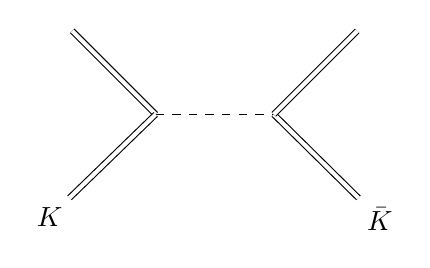
\begin{tikzpicture}
    \begin{feynman}
      \vertex (i);
      \vertex [right=of i] (m);
      \vertex [above right=of m] (f1);
      \vertex [below right=of m] (f2) {$\bar{K}$};
      \vertex [above left=of i] (s1);
      \vertex [below left=of i] (s2) {$K$};

      \diagram*{
        (i) -- [scalar] (m), % label ``meson''
        (f2) -- [double distance=1.5pt] (m) -- [double distance=1.5pt] (f1), % make these double lines
        (s1) -- [double distance=1.5pt] (i) -- [double distance=1.5pt] (s2),
      };
    \end{feynman}
  \end{tikzpicture}
\end{center}
%This is an effective diagram leading to a Yukawa force in $1 + 1$ dimensions, which decays exponentially with separation $s$.
%
%The amplitude of the tail of the of the soliton kink is $A = 2$. The factor of $32$ in the force ultimately comes from the mass being $m = 2$. More generally, one can show that if we put in parameters into our theory, we have
%\[
% F = 2 m^2 A^2 e^{-ms}.
%\]

So what happens to this soliton? The force we derived was positive. So the kink is made to move to the right. By symmetry, we will expect the anti-kink to move towards the left. They will collide!

What happens when they collide? All our analysis so far assumed the kinks were well-separated, so everything breaks down. We can only understand this phenomenon numerically. After doing some numerical simulations, we see that there are two regimes:
\begin{itemize}
  \item If the kinks are moving slowly, then they will annihilate into \emph{meson radiation}.
  \item If the kinks are moving very quickly, then they often bounce off each other.
\end{itemize}
%We can now study the time-dependence. The kinks will accelerate due to standard Newtonian dynamics, and they will move towards each other. However, the full dynamics of the kink-antikink pair is complicated. When they hit each other, they annihilate, and this happens in the regime where the separation is large. Where does the energy go when they annihilate? The answer is that they annihilate into meson radiation, which we can discover by doing numerical simulations.
%
%Annihilation is what happens if they are initially at rest, or slowly moving. However, at high speed, they happen to bounce of each other (of course, there is still some energy loss to radiation). These are very complicated, and we understand this mostly through numerical simulations.

\subsection{Quantization of kink motion}
We now briefly talk about how to quantize kinks. The most naive way of doing so is pretty straightforward. We use the moduli space approximation, and then we have a very simple kink Lagrangian.
\[
  L = \frac{1}{2} M \dot{a}^2.
\]
This is just a free particle moving in $\R$ with mass $M$. This $a$ is known as the \term{collective coordinate} of the kink. Quantizing a free particle is very straightforward. It is just IB Quantum Mechanics. For completeness, we will briefly outline this procedure.

We first put the system in Hamiltonian form. The conjugate momentum to $a$ is given by
\[
  P = M \dot{a}.
\]
Then the Hamiltonian is given by
\[
  H = P \dot{a} - L = \frac{1}{2M} P^2.
\]
Then to quantize, we replace $P$ by the operator $-i\hbar \frac{\partial}{\partial a}$. In this case, the quantum Hamiltonian is given by
\[
  H = - \frac{\hbar^2}{2M} \frac{\partial^2}{\partial a^2}.
\]
A wavefunction is a function of $a$ and $t$, and this is just ordinary QM for a single particle.

As usual, the stationary states are given by
\[
  \psi(a) = e^{i\kappa a},
\]
and the momentum and energy (eigenvalues) are
\[
  P = \hbar \kappa,\quad H = E = \frac{\hbar^2 \kappa^2}{2M} = \frac{P^2}{2M}.
\]

Is this actually ``correct''? Morally speaking, we really should quantize the complete $1 + 1$ dimensional field theory. What would this look like?

In normal quantum field theory, we consider perturbations around a vacuum solution, say $\phi \equiv 1$, and we obtain mesons. Here if we want to quantize the kink solution, we should consider field oscillations around the kink. Then the solution contains both a kink and a meson. These mesons give rise to quantum corrections to the kink mass $M$.

Should we be worried about these quantum corrections? Unsurprisingly, it turns out these quantum corrections are of the order of the meson mass. So we should not be worried when the meson mass is small.

Meson-kink scattering can also be studied in the full quantum theory. To first approximation, since the kink is heavy, mesons are reflected or transmitted with some probabilities, while the momentum of the kink is unchanged. But when we work to higher orders, then of course the kink will move as a result. This is all rather complicated.

For more details, see Rajaraman's \emph{Solitons and Instantons}, or Weinberg's \emph{Classical Solutions in Quantum Field Theory}.

The thing that is really hard to understand in the quantum field theory is kink-antikink pair production. This happens in meson collisions when the mesons are very fast, and the theory is highly relativistic. What we have done so far is perturbative and makes the non-relativistic approximation to get the adiabatic picture. It is \emph{very} difficult to understand the highly relativistic regime.

\subsection{Sine-Gordon kinks}
We end the section by briefly talking about kinks in a different theory, namely the \term{sine-Gordon theory}. In this theory, kinks are often known as \emph{solitons}\index{sine-Gordon soliton} instead.

The sine-Gordon theory is given by the potential
\[
  U(\phi) = 1 - \cos \phi.
\]
Again, we suppress coupling constants, but it is possible to add them back.

The potential looks like
\begin{center}
  \begin{tikzpicture}
    \draw [->](-3, 0) -- (3, 0) node [right] {$\phi$};
    \draw [->] (0, -0.5) -- (0, 2) node [above] {$U(\phi)$};

    \draw [mblue, thick] (0, 0) cos (0.3, 0.7) sin (0.6, 1.4) cos (0.9, 0.7) sin (1.2, 0) cos (1.5, 0.7) sin (1.8, 1.4) cos (2.1, 0.7) sin (2.4, 0) cos (2.7, 0.7) sin (3, 1.4);;
    \draw [mblue, thick, xscale=-1] (0, 0) cos (0.3, 0.7) sin (0.6, 1.4) cos (0.9, 0.7) sin (1.2, 0) cos (1.5, 0.7) sin (1.8, 1.4) cos (2.1, 0.7) sin (2.4, 0) cos (2.7, 0.7) sin (3, 1.4);;

    \node at (1.2, 0) [below] {$2\pi$};
    \node at (2.4, 0) [below] {$4\pi$};
    \node at (-1.2, 0) [below] {$2\pi$};
    \node at (-2.4, 0) [below] {$4\pi$};
  \end{tikzpicture}
\end{center}
Now there are \emph{infinitely many} distinct vacua. In this case, we find we need to pick $W$ such that
\[
  \frac{\d W}{\d \phi} = 2 \sin \frac{1}{2}\phi.
\]

\subsubsection*{Static sine-Gordon kinks}
To find the static kinks in the sine-Gordon theory, we again look at the Bogomolny equation. We have to solve
\[
  \frac{\d \phi}{\d x} = 2 \sin \frac{1}{2}\phi.
\]
This can be solved. This involves integrating a $\csc$, and ultimately gives us a solution
\[
  \phi(x) = 4 \tan^{-1} e^{x - a}.
\]
We can check that this solution interpolates between $0$ and $2\pi$.

\begin{center}
  \begin{tikzpicture}
    \draw [->] (-4, 0) -- (4, 0) node [right] {$x$};
    \draw [->] (0, -0.5) -- (0, 2.5) node [above] {$\phi$};

    \draw [mblue, thick] plot [smooth] coordinates {(-4.0,0.00000) (-3.9,0.00000) (-3.8,0.00000) (-3.7,0.00001) (-3.6,0.00001) (-3.5,0.00001) (-3.4,0.00001) (-3.3,0.00002) (-3.2,0.00002) (-3.1,0.00003) (-3.0,0.00005) (-2.9,0.00006) (-2.8,0.00008) (-2.7,0.00011) (-2.6,0.00015) (-2.5,0.00020) (-2.4,0.00027) (-2.3,0.00037) (-2.2,0.00050) (-2.1,0.00068) (-2.0,0.00091) (-1.9,0.00123) (-1.8,0.00166) (-1.7,0.00224) (-1.6,0.00303) (-1.5,0.00409) (-1.4,0.00552) (-1.3,0.00745) (-1.2,0.01005) (-1.1,0.01357) (-1.0,0.01831) (-0.9,0.02472) (-0.8,0.03336) (-0.7,0.04502) (-0.6,0.06074) (-0.5,0.08190) (-0.4,0.11035) (-0.3,0.14847) (-0.2,0.19922) (-0.1,0.26607) (0.0,0.35251) (0.1,0.46091) (0.2,0.59053) (0.3,0.73548) (0.4,0.88474) (0.5,1.02559) (0.6,1.14850) (0.7,1.24946) (0.8,1.32902) (0.9,1.39011) (1.0,1.43628) (1.1,1.47087) (1.2,1.49666) (1.3,1.51583) (1.4,1.53006) (1.5,1.54061) (1.6,1.54843) (1.7,1.55423) (1.8,1.55852) (1.9,1.56170) (2.0,1.56406) (2.1,1.56580) (2.2,1.56710) (2.3,1.56806) (2.4,1.56877) (2.5,1.56929) (2.6,1.56968) (2.7,1.56997) (2.8,1.57019) (2.9,1.57034) (3.0,1.57046) (3.1,1.57055) (3.2,1.57061) (3.3,1.57066) (3.4,1.57070) (3.5,1.57072) (3.6,1.57074) (3.7,1.57076) (3.8,1.57077) (3.9,1.57077) (4.0,1.57078)};
    % map (\x -> (showFFloat (Just 1) x "", showFFloat (Just 5) (atan ( exp (3*x - 1))) "")) [-4,-3.9..4]

    \draw [dashed] (-4, 1.57078) -- (4, 1.57078);

    \node [left] at (-4, 0) {$0$};
    \node [right] at (4, 1.57078) {$2\pi$};
    \node [circ] at (0.33, 0.785398) {};
    \draw [dashed] (0.33, 0.785398) -- (0.33, 0) node [below] {$a$};
  \end{tikzpicture}
\end{center}

Unlike the $\phi^4$ theory, dynamical multi-kink solutions exist here and can be derived \emph{exactly}. One of the earlier ways to do so was via B\"acklund transforms, but that was very complicated. People later invented better methods, but they are still not very straightforward. Nevertheless, it can be done. Ultimately, this is due to the sine-Gordon equation being \emph{integrable}. For more details, refer to the IID Integrable Systems course.

\begin{eg}
  There is a two-kink solution
  \[
    \phi (x, t) = 4 \tan^{-1} \left(\frac{v \sinh \gamma x}{ \cosh \gamma vt}\right),
  \]
  where, as usual, we have
  \[
    \gamma = (1 - v^2)^{-1/2}.
  \]
  For $v = 0.01$, this looks like
  \begin{center}
    \begin{tikzpicture}
      \draw [->] (-4, 0) -- (4, 0) node [right] {$x$};
      \draw [->] (0, -2.5) -- (0, 2.5) node [above] {$\phi$};

      \draw [mblue, thick] plot [smooth] coordinates {(-4.0,-1.56957) (-3.9,-1.56914) (-3.8,-1.56856) (-3.7,-1.56778) (-3.6,-1.56672) (-3.5,-1.56529) (-3.4,-1.56337) (-3.3,-1.56077) (-3.2,-1.55726) (-3.1,-1.55252) (-3.0,-1.54613) (-2.9,-1.53751) (-2.8,-1.52587) (-2.7,-1.51019) (-2.6,-1.48906) (-2.5,-1.46067) (-2.4,-1.42263) (-2.3,-1.37197) (-2.2,-1.30524) (-2.1,-1.21893) (-2.0,-1.11067) (-1.9,-0.98117) (-1.8,-0.83628) (-1.7,-0.68699) (-1.6,-0.54603) (-1.5,-0.42296) (-1.4,-0.32183) (-1.3,-0.24211) (-1.2,-0.18089) (-1.1,-0.13458) (-1.0,-0.09986) (-0.9,-0.07394) (-0.8,-0.05461) (-0.7,-0.04020) (-0.6,-0.02942) (-0.5,-0.02129) (-0.4,-0.01509) (-0.3,-0.01027) (-0.2,-0.00637) (-0.1,-0.00305) (0.0,0.00000) (0.1,0.00305) (0.2,0.00637) (0.3,0.01027) (0.4,0.01509) (0.5,0.02129) (0.6,0.02942) (0.7,0.04020) (0.8,0.05461) (0.9,0.07394) (1.0,0.09986) (1.1,0.13458) (1.2,0.18089) (1.3,0.24211) (1.4,0.32183) (1.5,0.42296) (1.6,0.54603) (1.7,0.68699) (1.8,0.83628) (1.9,0.98117) (2.0,1.11067) (2.1,1.21893) (2.2,1.30524) (2.3,1.37197) (2.4,1.42263) (2.5,1.46067) (2.6,1.48906) (2.7,1.51019) (2.8,1.52587) (2.9,1.53751) (3.0,1.54613) (3.1,1.55252) (3.2,1.55726) (3.3,1.56077) (3.4,1.56337) (3.5,1.56529) (3.6,1.56672) (3.7,1.56778) (3.8,1.56856) (3.9,1.56914) (4.0,1.56957)};
      \draw [mred, thick] plot [smooth] coordinates {(-4.0,-1.53726) (-3.9,-1.52555) (-3.8,-1.50975) (-3.7,-1.48847) (-3.6,-1.45988) (-3.5,-1.42157) (-3.4,-1.37057) (-3.3,-1.30340) (-3.2,-1.21659) (-3.1,-1.10779) (-3.0,-0.97784) (-2.9,-0.83269) (-2.8,-0.68347) (-2.7,-0.54286) (-2.6,-0.42031) (-2.5,-0.31974) (-2.4,-0.24053) (-2.3,-0.17975) (-2.2,-0.13381) (-2.1,-0.09939) (-2.0,-0.07374) (-1.9,-0.05467) (-1.8,-0.04052) (-1.7,-0.03002) (-1.6,-0.02224) (-1.5,-0.01648) (-1.4,-0.01221) (-1.3,-0.00904) (-1.2,-0.00670) (-1.1,-0.00496) (-1.0,-0.00367) (-0.9,-0.00271) (-0.8,-0.00200) (-0.7,-0.00147) (-0.6,-0.00108) (-0.5,-0.00078) (-0.4,-0.00055) (-0.3,-0.00038) (-0.2,-0.00023) (-0.1,-0.00011) (0.0,0.00000) (0.1,0.00011) (0.2,0.00023) (0.3,0.00038) (0.4,0.00055) (0.5,0.00078) (0.6,0.00108) (0.7,0.00147) (0.8,0.00200) (0.9,0.00271) (1.0,0.00367) (1.1,0.00496) (1.2,0.00670) (1.3,0.00904) (1.4,0.01221) (1.5,0.01648) (1.6,0.02224) (1.7,0.03002) (1.8,0.04052) (1.9,0.05467) (2.0,0.07374) (2.1,0.09939) (2.2,0.13381) (2.3,0.17975) (2.4,0.24053) (2.5,0.31974) (2.6,0.42031) (2.7,0.54286) (2.8,0.68347) (2.9,0.83269) (3.0,0.97784) (3.1,1.10779) (3.2,1.21659) (3.3,1.30340) (3.4,1.37057) (3.5,1.42157) (3.6,1.45988) (3.7,1.48847) (3.8,1.50975) (3.9,1.52555) (4.0,1.53726)};
      % let v = 0.01 in let g = sqrt (1 / (1 - v * v)) in let t = 400 in map (\x -> (showFFloat (Just 1) x "", showFFloat (Just 5) (atan (v * sinh (g * x * 3) / cosh (v * g * t))) "")) [-4,-3.9..4]

      \draw [dashed] (-4, 1.57078) -- (4, 1.57078);
      \draw [dashed] (-4, -1.57078) -- (4, -1.57078);

      \node [right] at (4, 1.57078) {$2\pi$};
      \node [left] at (-4, -1.57078) {$-2\pi$};

      \node [mblue, left] at (1.73, 0.785) {\small$t = 0$};
      \node [mred, right] at (2.85, 0.785) {\small$t = \pm400$};
    \end{tikzpicture}
  \end{center}

  Note that since $\phi(x, t) = \phi(x, -t)$, we see that this solution involves two solitons at first approaching each other, and then later bouncing off. Thus, the two kinks \emph{repel} each other. When we did kinks in $\phi^4$ theory, we saw that a kink and an anti-kink attracted, but here there are two kinks, which is qualitatively different.

  We can again compute the force just like the $\phi^4$ theory, but alternatively, since we have a full, exact solution, we can work it out directly from the solution! The answers, fortunately, agree. If we do the computations, we find that the point of closest approach is $\sim 2 \log \left(\frac{2}{v}\right)$ if $v$ is small.
\end{eg}

There are some important comments to make. In the sine-Gordon theory, we can have very complicated interactions between kinks and anti-kinks, and these can connect vastly different vacua. However, \emph{static} solutions must join $2n\pi$ and $2(n \pm 1)\pi$ for some $n$, because if we want to join vacua further apart, we will have more than one kink, and they necessarily interact.

If we have multiple kinks and anti-kinks, then each of these things can have their own velocity, and we might expect some very complicated interaction between them, such as annihilation and pair production. But remarkably, the interactions are \emph{not} complicated. If we try to do numerical simulations, or use the exact solutions, we see that we do not have energy loss due to ``radiation''. Instead, the solitons remain very well-structured and retain their identities. This, again, is due to the theory being integrable.

\subsubsection*{Topology of the sine-Gordon equation}
There are also a lot of interesting things we can talk about without going into details about what the solutions look like.

The important realization is that our potential is periodic in $\phi$. For the sine-Gordon theory, it is much better to think of this as a field modulo $2\pi$, i.e.\ as a function
\[
  \phi: \R \to S^1.
\]
In this language, the boundary condition is that $\phi(x) = 0 \bmod 2\pi$ as $x \to \pm \infty$. Thus, instead of thinking of the kink as joining two vacua, we can think of it as ``winding around the circle'' instead.

We can go further. Since the boundary conditions of $\phi$ are now the same on two sides, we can join the ends of the domain $\R$ together, and we can think of $\phi$ as a map
\[
  \phi: S^1 \to S^1
\]
instead. This is a \term{compactification} of space.

Topologically, such maps are classified by their \term{winding number}, or the \term{degree}, which we denote \term{$Q$}. This is a topological (homotopy) invariant of a map, and is preserved under continuous deformations of the field. Thus, it is preserved under time evolution of the field.

Intuitively, the winding number is just how many times we go around the circle. There are multiple (equivalent) ways of making this precise.

The first way, which is the naive way, is purely topological. We simply have to go back to the first picture, where we regard $\phi$ as a real value. Suppose the boundary values are
\[
  \phi(-\infty) = 2 n_- \pi,\quad \phi(\infty) = 2 n_+ \pi.
\]
Then we set the winding number to be $Q = n_+ - n_-$.

Topologically, we are using the fact that $\R$ is the \term{universal covering space}\index{covering space} of the circle, and thus we are really looking at the induced map on the fundamental group of the circle.

\begin{eg}
  As we saw, a single kink has $Q = 1$.
  \begin{center}
    \begin{tikzpicture}
      \draw [->] (-4, 0) -- (4, 0) node [right] {$x$};
      \draw [->] (0, -0.5) -- (0, 2.5) node [above] {$\phi$};

      \draw [mblue, thick] plot [smooth] coordinates {(-4.0,0.00000) (-3.9,0.00000) (-3.8,0.00000) (-3.7,0.00001) (-3.6,0.00001) (-3.5,0.00001) (-3.4,0.00001) (-3.3,0.00002) (-3.2,0.00002) (-3.1,0.00003) (-3.0,0.00005) (-2.9,0.00006) (-2.8,0.00008) (-2.7,0.00011) (-2.6,0.00015) (-2.5,0.00020) (-2.4,0.00027) (-2.3,0.00037) (-2.2,0.00050) (-2.1,0.00068) (-2.0,0.00091) (-1.9,0.00123) (-1.8,0.00166) (-1.7,0.00224) (-1.6,0.00303) (-1.5,0.00409) (-1.4,0.00552) (-1.3,0.00745) (-1.2,0.01005) (-1.1,0.01357) (-1.0,0.01831) (-0.9,0.02472) (-0.8,0.03336) (-0.7,0.04502) (-0.6,0.06074) (-0.5,0.08190) (-0.4,0.11035) (-0.3,0.14847) (-0.2,0.19922) (-0.1,0.26607) (0.0,0.35251) (0.1,0.46091) (0.2,0.59053) (0.3,0.73548) (0.4,0.88474) (0.5,1.02559) (0.6,1.14850) (0.7,1.24946) (0.8,1.32902) (0.9,1.39011) (1.0,1.43628) (1.1,1.47087) (1.2,1.49666) (1.3,1.51583) (1.4,1.53006) (1.5,1.54061) (1.6,1.54843) (1.7,1.55423) (1.8,1.55852) (1.9,1.56170) (2.0,1.56406) (2.1,1.56580) (2.2,1.56710) (2.3,1.56806) (2.4,1.56877) (2.5,1.56929) (2.6,1.56968) (2.7,1.56997) (2.8,1.57019) (2.9,1.57034) (3.0,1.57046) (3.1,1.57055) (3.2,1.57061) (3.3,1.57066) (3.4,1.57070) (3.5,1.57072) (3.6,1.57074) (3.7,1.57076) (3.8,1.57077) (3.9,1.57077) (4.0,1.57078)};
    % map (\x -> (showFFloat (Just 1) x "", showFFloat (Just 5) (atan ( exp (3*x - 1))) "")) [-4,-3.9..4]

      \draw [dashed] (-4, 1.57078) -- (4, 1.57078);

      \node [left] at (-4, 0) {$0$};
      \node [right] at (4, 1.57078) {$2\pi$};
    \end{tikzpicture}
  \end{center}
\end{eg}

Thus, we can think of the $Q$ as the \emph{net soliton number}.


But this construction we presented is rather specific to maps from $S^1$ to $S^1$. We want something more general that can be used for more complicated systems. We can do this in a more ``physics'' way. We note that there is a \emph{topological} current
\[
  j^\mu = \frac{1}{2\pi} \varepsilon^{\mu\nu} \partial_\nu \phi,
\]
where $\varepsilon^{\mu\nu}$ is the anti-symmetric tensor in $1 + 1$ dimensions, chosen so that $\varepsilon^{01} = 1$.

In components, this is just
\[
  j^\mu = \frac{1}{2\pi} (\partial_x \phi, - \partial_t \phi).
\]
This is conserved because of the symmetry of mixed partial derivatives, so that
\[
  \partial_\mu j^\mu = \frac{1}{2\pi} \varepsilon^{\mu\nu} \partial_\mu \partial_\nu \phi = 0.
\]
As usual, a current induces a conserved charge
\[
  Q = \int_{-\infty}^\infty j^0 \;\d x = \frac{1}{2\pi} \int_{-\infty}^\infty \partial_x \phi \;\d x = \frac{1}{2\pi} (\phi(\infty) - \phi(-\infty)) = n_+ - n_-,
\]
which is the formula we had earlier.

Note that all these properties do not depend on $\phi$ satisfying any field equations! It is completely topological.

Finally, there is also a differential geometry way of defining $Q$. We note that the target space $S^1$ has a normalized volume form $\omega$ so that
\[
  \int_{S^1} \omega = 1.
\]
For example, we can take
\[
  \omega = \frac{1}{2\pi}\;\d \phi.
\]
Now, given a mapping $\phi: \R \to S^1$, we can pull back the volume form to obtain
\[
  \phi^* \omega = \frac{1}{2\pi} \frac{\d \phi}{\d x} \;\d x.
\]
We can then define the degree of the map to be
\[
  Q = \int \phi^* \omega = \frac{1}{2\pi}\int_{-\infty}^\infty \frac{\d \phi}{\d x}\;\d x.
\]
This is exactly the same as the formula we obtained using the current!

Note that even though the volume form is normalized on $S^1$ and has integral $1$, the integral when pulled back is not $1$. We can imagine this as saying if we wind around the circle $n$ times, then after pulling back, we would have pulled back $n$ ``copies'' of the volume form, and so the integral will be $n$ times that of the integral on $S^1$.

We saw that these three definitions gave the same result, and different definitions have different benefits. For example, in the last two formulations, it is not \emph{a priori} clear that the winding number has to be an integer, while this is clear in the first formulation.

\section{Vortices}
We are now going to start studying \emph{vortices}. These are topological solitons in two space dimensions. While we mostly studied $\phi^4$ kinks last time, what we are going to do here is more similar to the sine-Gordon theory than the $\phi^4$ theory, as it is largely topological in nature.

A lot of the computations we perform in the section are much cleaner when presented using the language of differential forms. However, we shall try our best to provide alternative versions in coordinates for the easily terrified.

\subsection{Topological background}
\subsubsection*{Sine-Gordon kinks}
We now review what we just did for sine-Gordon kinks, and then try to develop some analogous ideas in higher dimension. The sine-Gordon equation is given by
\[
  \frac{\partial^2 \theta}{\partial t^2} - \frac{\partial^2 \theta}{\partial x^2} + \sin \theta = 0.
\]

We want to choose boundary conditions so that the energy has a chance to be finite. The first part is, of course, to figure out what the energy is. The energy-momentum conservation equation given by Noether's theorem is
\[
  \partial_t \left(\frac{\theta_t^2 + \theta_x^2}{2} + (1 - \cos \theta)\right) + \partial_x (-\theta_t \theta_x) = \partial_\mu P^\mu = 0.
\]
The energy we will be considering is thus
\[
  E = \int_{\R} P^0 \;\d x = \int_\R \left(\frac{\theta_t^2 + \theta_x^2}{2} + (1 - \cos \theta)\right)\;\d x.
\]
Thus, to obtain finite energy, we will want $\theta(x) \to 2n_{\pm} \pi$ for some integers $n_{\pm}$ as $x \to \pm \infty$. What is the significance of this $n_{\pm}$?
\begin{eg}
  Consider the basic kink
  \[
    \theta_K(x) = 4\tan^{-1} e^x.
  \]
  Picking the standard branch of $\tan^{-1}$, this kink looks like
  \begin{center}
    \begin{tikzpicture}
      \draw [->] (-4, 0) -- (4, 0) node [right] {$x$};
      \draw [->] (0, -0.5) -- (0, 2.5) node [above] {$\phi$};

      \draw [mblue, thick] plot [smooth] coordinates {(-4.0,0.00001) (-3.9,0.00001) (-3.8,0.00001) (-3.7,0.00002) (-3.6,0.00002) (-3.5,0.00003) (-3.4,0.00004) (-3.3,0.00005) (-3.2,0.00007) (-3.1,0.00009) (-3.0,0.00012) (-2.9,0.00017) (-2.8,0.00022) (-2.7,0.00030) (-2.6,0.00041) (-2.5,0.00055) (-2.4,0.00075) (-2.3,0.00101) (-2.2,0.00136) (-2.1,0.00184) (-2.0,0.00248) (-1.9,0.00335) (-1.8,0.00452) (-1.7,0.00610) (-1.6,0.00823) (-1.5,0.01111) (-1.4,0.01499) (-1.3,0.02024) (-1.2,0.02732) (-1.1,0.03687) (-1.0,0.04975) (-0.9,0.06710) (-0.8,0.09047) (-0.7,0.12185) (-0.6,0.16382) (-0.5,0.21953) (-0.4,0.29255) (-0.3,0.38616) (-0.2,0.50193) (-0.1,0.63760) (0.0,0.78540) (0.1,0.93320) (0.2,1.06887) (0.3,1.18464) (0.4,1.27824) (0.5,1.35126) (0.6,1.40698) (0.7,1.44895) (0.8,1.48033) (0.9,1.50369) (1.0,1.52105) (1.1,1.53393) (1.2,1.54348) (1.3,1.55056) (1.4,1.55580) (1.5,1.55969) (1.6,1.56257) (1.7,1.56470) (1.8,1.56628) (1.9,1.56745) (2.0,1.56832) (2.1,1.56896) (2.2,1.56944) (2.3,1.56979) (2.4,1.57005) (2.5,1.57024) (2.6,1.57039) (2.7,1.57049) (2.8,1.57057) (2.9,1.57063) (3.0,1.57067) (3.1,1.57070) (3.2,1.57073) (3.3,1.57075) (3.4,1.57076) (3.5,1.57077) (3.6,1.57078) (3.7,1.57078) (3.8,1.57079) (3.9,1.57079) (4.0,1.57079)};
    % map (\x -> (showFFloat (Just 1) x "", showFFloat (Just 5) (atan ( exp (3*x - 1))) "")) [-4,-3.9..4]

      \draw [dashed] (-4, 1.57078) -- (4, 1.57078);

      \node [left] at (-4, 0) {$0$};
      \node [right] at (4, 1.57078) {$2\pi$};
    \end{tikzpicture}
  \end{center}
  This goes from $\theta = 0$ to $\theta = 2\pi$.
\end{eg}

To better understand this, we can think of $\theta$ as an angular variable, i.e.\ we identify $\theta \sim \theta + 2n\pi$ for any $n \in \Z$. This is a sensible thing because the energy density and the equation etc.\ are unchanged when we shift everything by $2n\pi$. Thus, $\theta$ is not taking values in $\R$, but in $\R/2\pi\Z \cong S^1$.

Thus, for each fixed $t$, our field $\theta$ is a map
\[
  \theta: \R \to S^1.
\]
The number $Q = n_+ - n_-$ equals the number of times $\theta$ covers the circle $S^1$ on going from $x = -\infty$ to $x = +\infty$. This is the winding number, which is interpreted as the topological charge.

As we previously discussed, we can express this topological charge as the integral of some current. We can write
\[
  Q = \frac{1}{2\pi} \int_{\theta(\R)} \d \theta = \frac{1}{2\pi} \int_{-\infty}^\infty \frac{\d \theta}{\d x}\;\d x.
\]
Note that this formula automatically takes into account the orientation. This is the form that will lead to generalization in higher dimensions.

This function $\frac{\d \theta}{\d x}$ appearing in the integral has the interpretation as a topological charge density. Note that there is a topological conservation law
\[
  \partial_\mu j^\mu = \frac{\partial j^0}{\partial t} + \frac{\partial j^1}{\partial x} = 0,
\]
where
\[
  j^0 = \theta_x,\quad j^1 = -\theta_t.
\]
This conservation law is not a consequence of the field equations, but merely a mathematical identity, namely the commutation of partial derivatives.

\subsubsection*{Two dimensions}
For the sine-Gordon kink, the target space was a circle $S^1$. Now, we are concerned with the \term{unit disk}\index{$D$}
\[
  D = \{(x^1, x^2): |\mathbf{x}|^2 < 1\} \subseteq \R^2.
\]
We will then consider fields
\[
  \Phi: D \to D.
\]
In the case of a sine-Gordon kink, we still cared about moving solitons. However, here we will mostly work with static solutions, and study fields at a fixed time. Thus, there is no time variable appearing.

Using the canonical isomorphism $\R^2 \cong \C$, we can think of the target space as the unit disk in the complex plane, and write the field as
\[
  \Phi = \Phi^1 + i \Phi^2.
\]
However, we will usually view the $D$ in the domain as a real space instead.

We will impose some boundary conditions. We pick any function $\chi: S^1 \to \R$, and consider
\[
  g = e^{i\chi}: S^1 \to S^1 = \partial D \subseteq D.
\]
Here $g$ is a genuine function, and has to be single-valued. So $\chi$ must be single-valued modulo $2\pi$. We then require
\[
  \Phi_{\partial D} = g = e^{i \chi}.
\]
In particular, $\Phi$ must send the boundary to the boundary.

Now the target space $D$ has a canonical choice of measure $\d \Phi^1 \wedge \d \Phi^2$. Then we can expect the new topological charge to be given by
\[
  Q = \frac{1}{\pi} \int_D \d \Phi^1 \wedge \d \Phi^2 = \frac{1}{\pi} \int_D \det
  \begin{pmatrix}
    \frac{\partial \Phi^1}{\partial x^1} & \frac{\partial \Phi^1}{\partial x^2}\\
    \frac{\partial \Phi^2}{\partial x^1} & \frac{\partial \Phi^2}{\partial x^2}
  \end{pmatrix}\;\d x^1 \wedge \d x^2.
\]
Thus, the charge density is given by
\[
  j^0 = \frac{1}{2} \varepsilon_{ab} \varepsilon_{ij} \frac{\partial \Phi^a}{\partial x^i} \frac{\partial \Phi^b}{\partial x^j}.
\]
Crucially, it turns out this charge density is a total derivative, i.e.\ we have
\[
  j^0 = \frac{\partial V^i}{\partial x^i}
\]
for some function $V$. It is not immediately obvious this is the case. However, we can in fact pick
\[
  V^i = \frac{1}{2} \varepsilon_{ab}\varepsilon^{ij} \Phi^a \frac{\partial \Phi^b}{\partial x^j}.
\]
To see this actually works, we need to use the anti-symmetry of $\varepsilon^{ij}$ and observe that
\[
  \varepsilon^{ij} \frac{\partial^2 \Phi^b}{\partial x^i \partial x^j} = 0.
\]
Equivalently, using the language of differential forms, we view the charge density $j^0$ as the $2$-form
\[
  j^0 = \d \Phi^1 \wedge \d \Phi^2 = \d (\Phi^1\;\d \Phi^2) = \frac{1}{2} \d (\Phi^1 \;\d \Phi^2 - \Phi^2 \;\d \Phi^1).
\]
By the divergence theorem, we find that
\[
  Q = \frac{1}{2\pi}\oint_{\partial D} \Phi^1 \;\d \Phi^2 - \Phi^2 \;\d \Phi^1.
\]
We then use that on the boundary,
\[
  \Phi^1 = \cos \chi,\quad \Phi^2 = \sin \chi,
\]
so
\[
  Q = \frac{1}{2\pi} \oint_{\partial D} (\cos^2 \chi + \sin^2 \chi) \;\d \chi = \frac{1}{2\pi} \oint_{\partial D} \;\d \chi = N.
\]
Thus, the charge is just the winding number of $g$!

%But what actually is the degree telling us? Let's fix a boundary condition $\Phi|_{\partial D} = g = e^{i\chi}$, where $\chi: \partial D \cong S^1 \to \R$ is a real function. Since $g$ is now a map from the boundary circle to the boundary circle. So $g$ itself has got a winding number,
%\[
% \frac{1}{2\pi} \int_0^{2\pi} \frac{\d \chi}{\d \theta} \;\d \theta.
%\]
%Let's relate the degree of $\Phi$ to the winding number of $g$. To do so, we will need the fact that the Jacobian determinant is a total derivative, so that we can apply Green's identity. Thus, we want to write $j^0$ as
%\[
% j^0 = \frac{\partial V^i}{\partial x^i}
%\]
%for some $V^i$. It might not be immediately obvious how we can pick such a $V^i$, but notice that
%\[
% \varepsilon_{ij} \frac{\partial^2 \Phi^b}{\partial x^i \partial x^j} = 0
%\]
%by anti-symmetry. So we can in fact pick
%\[
% V^i = \frac{1}{2} \varepsilon_{ab}\varepsilon_{ij} \Phi^a \frac{\partial \Phi^b}{\partial x^j}.
%\]
%Then in this case, we have
%\[
% \int_D j^0 \;\d x = \int \left(\frac{\partial V^1}{\partial x^1} + \frac{\partial V^2}{\partial x^2}\right)\;\d x^1 \;\d x^2 = \oint_{\partial D} V^1 \;\d x^2 - V^2 \;\d x^1.
%\]
%On the boundary, we know $\Phi^1 = \cos \chi$ and $\Phi^2 = \sin \chi$. Substituting that in, we can calculate $V^1$ and $V^2$ on the boundary, and then work out the integral to be
%\[
% \int_D j\;\d x = \frac{1}{2} \oint_D \;\d \chi = \pi N,
%\]
%where $N$ is the winding number of $g: S^1 \to S^1$.
%
%This is a general phenomenon. Often, the appearance of anti-symmetric combinations of derivatives will allow us to reduce complicated quantities into total derivatives. Then this will allow us to relate things that \emph{a priori} depends on the value of $\Phi$ everywhere into something that depends only on the boundary values.
%The next interesting thing to notice is that the charge $Q$ is invariant under scaling of the domain. If we scale $x$ by $R$, then $\d x^1 \wedge \d x^2$ gets scaled up by $R^2$, but the Jacobian gets scaled down by $R^2$. Thus, an interesting thing to do is to take take $R \to \infty$. Then the domain becomes all of $\R^2$.

Now notice that our derivation didn't really depend on our domain being $D$. It could have been any region bounded by a simple closed curve in $\R^2$. In particular, we can take it to be a disk $D_R$ of arbitrary radius $R$.

What we are \emph{actually} interested in is a field
\[
  \Phi: \R^2 \to D.
\]
We then impose asymptotic boundary conditions
\[
  \Phi \sim g = e^{i\chi}
\]
as $|x| \to \infty$. We can still define the charge or degree by
\[
  Q = \frac{1}{\pi} \int_{\R^2} j^0 \;\d x^1 \;\d x^2 = \frac{1}{\pi} \lim_{R \to \infty}\int_{D_R} j^0 \;\d x^1 \;\d x^2
\]
This is then again the winding number of $g$.
%So our field is now a mapping $\Phi: \R^2 \to D$. We then set the asymptotic boundary condition $\Phi \sim g = e^{i \chi}$ as $|x| \to \infty$. For these maps, we have the same formula for degree, namely
%\[
% Q = \frac{1}{\pi} \int_{\R^2} \frac{1}{2} \varepsilon_{ab} \varepsilon_{ij} \partial_i \Phi^a \partial_j \Phi^b \;\d x^1 \;\d x^2 = \frac{1}{2\pi} \lim_{R\to \infty} \oint_{|x| = R} \d \chi \in \Z.
%\]
%This is going to be our basic topological quantity for the vortices. Its existence, and being non-zero, is what gives rise to a stable vortex.

It is convenient to rewrite this in terms of an inner product. $\R^2$ itself has an inner product, and under the identification $\R^2 \cong \C$, the inner product can be written as
\[
  (a, b) = \frac{\bar{a} b + a \bar{b}}{2}.
\]
Use of this expression allows calculations to be done efficiently if one makes use of the fact that for real numbers $a$ and $b$, we have
\[
  (a, b) = (ai, bi) = ab, \quad (ai, b) = (a, bi) = 0.
\]
In particular, we can evaluate
\[
  (i \Phi, \d \Phi) = (i \Phi^1 - \Phi^2, \d \Phi^1 + i \d \Phi^2) = \Phi^1\;\d \Phi^2 - \Phi^2\;\d \Phi^1.
\]
This is just (twice) the current $V$ we found earlier! So we can write our charge as
\[
  Q = \frac{1}{2\pi} \lim_{R \to \infty} \oint_{|x| = R} (i \Phi, \d \Phi).
\]
We will refer to $(i \Phi, \d \Phi)$ as the current, and the corresponding charge density is $j^0 = \frac{1}{2} \d (i \Phi, \d \Phi)$.

%We can rewrite this in terms of complex numbers. Instead of viewing a $\Phi$ as a function valued in $D \subseteq \R^2$, we view it as a function $\Phi: D \to \C$. We already implicitly did so when we wrote the boundary condition as $e^{i \chi}$. In terms of complex numbers, we can write the standard inner product on $\R^2$ as
%\[
% (a, b) = \frac{\bar{a} b + a \bar{b}}{2}.
%\]
%Then we can write the integral for the charge as
%\[
% \oint_{\partial D}\;\d \chi = \oint_{\partial D} (i\Phi, \d \Phi).
%\]
%This formulation is sometimes more convenient for calculations.

This current is actually a familiar object from quantum mechanics: recall that for the Schr\"odinger's equation
\[
  i \frac{\partial \Phi}{\partial t} = - \frac{1}{2m} \Delta \Phi + V(x) \Phi,\quad \Delta = \nabla^2.
\]
the probability $\int |\Phi|^s \;\d x$ is conserved. The differential form of the probability conservation law is
\[
  \frac{1}{2} \partial_t (\Phi, \Phi) + \frac{1}{2m} \nabla \cdot (i \Phi, \nabla \Phi) = 0.
\]
What appears in the flux term here is just the topological current!

%The final comment, which we will not actually use, is that if we have a holomorphic function $f$, then consider the integral
%\[
% \frac{1}{2\pi i} \oint_C \frac{f'(z)}{f(z) - w}\;\d z.
%\]
%Using the residue theorem, we can see that this is the number of times $f$ takes value $w$, counted with multiplicity, within the area bounded by $C$. This is the \term{local degree} of the mapping. Indeed,
%\[
% \Res\left(\frac{f'(z)}{f(z) - w}, z_i\right) = n_i,
%\]
%where $f(z) - w = (z - z_i)^{n_i'} h(z)$, with $h(z_i) \not= 0$.
%
%But we can think about this in a different way. The integrand is an exact differential
%\[
% \frac{1}{2\pi i} [\log (f(z) - w)],
%\]
%and if we think about this carefully, this the change in argument of $f(z) - w$ around the curve.

\subsection{Global \texorpdfstring{$U(1)$}{U(1)} Ginzburg--Landau vortices}
We now put the theory into use. We are going to study \emph{Ginzburg--Landau vortices}\index{Ginzburg--Landau!vortex}. Our previous discussion involved a function taking values in the unit disk $D$. We will not impose such a restriction on our vortices. However, we will later see that any solution must take values in $D$.

The potential energy of the Ginzburg--Landau theory is given by
\[
  V(\Phi) = \frac{1}{2} \int_{\R^2} \left((\nabla \Phi, \nabla \Phi) + \frac{\lambda}{4} (1 - (\Phi, \Phi))^2 \right)\;\d x^1 \;\d x^2.
\]
where $\lambda > 0$ is some constant.

Note that the inner product is invariant under phase rotation, i.e.
\[
  (e^{i\chi} a, e^{i\chi}b) = (a, b)
\]
for $\chi \in \R$. So in particular, the potential satisfies
\[
  V(e^{i\chi}\Phi) = V(\Phi).
\]
Thus, our theory has a \term{global $\U(1)$ symmetry}\index{$\U(1)$ symmetry!global}.

The Euler--Lagrange equation of this theory says
\[
  - \Delta \Phi = \frac{\lambda}{2}(1 - |\Phi|^2) \Phi.
\]
This is the \emph{ungauged Ginzburg--Landau equation}\index{Ginzburg--Landau!ungauged}.

To justify the fact that our $\Phi$ takes values in $D$, we use the following lemma:
\begin{lemma}
  Assume $\Phi$ is a smooth solution of the ungauged Ginzburg--Landau equation in some domain. Then at any interior maximum point $x_*$ of $|\Phi|$, we have $|\Phi(x_*)| \leq 1$.
\end{lemma}

\begin{proof}
  Consider the function
  \[
    W(x) = 1 - |\Phi(x)|^2.
  \]
  Then we want to show that $W \geq 0$ when $W$ is minimized. We note that if $W$ is at a minimum, then the Hessian matrix must have non-negative eigenvalues. So, taking the trace, we must have $\Delta W(x_*) \geq 0$. Now we can compute $\Delta W$ directly. We have
  \begin{align*}
    \nabla W &= -2 (\Phi, \nabla \Phi)\\
    \Delta W &= \nabla^2 W \\
    &= - 2(\Phi, \Delta \Phi) - 2(\nabla \Phi, \nabla \Phi)\\
    &= \lambda |\Phi|^2 W - 2 |\nabla \Phi|^2.
  \end{align*}
  Thus, we can rearrange this to say
  \[
    2 |\nabla \Phi|^2 + \Delta W = \lambda |\Phi|^2 W.
  \]
  But clearly $2 |\nabla \Phi|^2 \geq 0$ everywhere, and we showed that $\Delta W(x_*) \geq 0$. So we must have $W(x_*) \geq 0$.
\end{proof}

By itself, this doesn't force $|\Phi| \in [0, 1]$, since we could imagine $|\Phi|$ having no maximum. However, if we prescribe boundary conditions such that $|\Phi| = 1$ on the boundary, then this would indeed imply that $|\Phi| \leq 1$ everywhere. Often, we can think of $\Phi$ as some ``complex order parameter'', in which case the condition $|\Phi| \leq 1$ is very natural.

The objects we are interested in are \emph{vortices}.

\begin{defi}[Ginzburg--Landau vortex]\index{Ginzburg--Landau!vortex}
  A global \emph{Ginzburg--Landau vortex} of charge $N > 0$ is a (smooth) solution of the ungauged Ginzburg--Landau equation of the form
  \[
    \Phi = f_N(r) e^{iN\theta}
  \]
  in polar coordinates $(r, \theta)$. Moreover, we require that $f_N(r) \to 1$ as $r \to \infty$.
\end{defi}
Note that for $\Phi$ to be a smooth solution, we must have $f_N(0) = 0$. In fact, a bit more analysis shows that we must have $f_N = O(r^N)$ as $r \to 0$. Solutions for $f_N$ do exist, and they look roughly like this:

\begin{center}
  \begin{tikzpicture}
    \draw [->] (-0.5, 0) -- (5, 0) node [right] {$r$};
    \draw [->] (0, -0.5) -- (0, 3) node [above] {$f_N$};

    \draw [mblue, thick, domain=0:5] plot [smooth] (\x, {2 * \x^4 / (1 + \x^4)});

    \draw [dashed] (-1, 2) -- (5, 2);

  \end{tikzpicture}
\end{center}

In the case of $N = 1$, we can visualize the field $\Phi$ as a vector field on $\C$. Then it looks like
\begin{center}
  \begin{tikzpicture}
    \draw [->] (-3, 0) -- (3, 0);
    \draw [->] (0, -3) -- (0, 3);

    \foreach \t in {0,30,60,90,120,150,180,210,240,270,300,330,360} {
      \begin{scope}[rotate=\t]
        \foreach \x in {0.5, 1, 1.5, 2, 2.5} {
          \pgfmathsetmacro\arlen{0.5 * (\x^4 / (1 + \x^4))^2}
          \draw [-latex'] (\x, 0) -- +(\arlen, 0);
        }
      \end{scope}
    }
  \end{tikzpicture}
\end{center}
This is known as a \emph{$2$-dimensional hedgehog}.

For general $N$, it might be more instructive to look at how the current looks like. Recall that the current is defined by $(i\Phi, \d \Phi)$. We can write this more explicitly as
\begin{align*}
  (i\Phi, \d \Phi) &= (if_N e^{iN\theta}, (\d f_N) e^{iN\theta} + i f_N N\;\d \theta e^{iN\theta})\\
  &= (if_N,\d f_N + i f_N N\;\d \theta).
\end{align*}
We note that $if_N$ and $\d f_N$ are orthogonal, while $i f_N$ and $i f_N N \d \theta$ are parallel. So the final result is
\[
  (i\Phi, \d \Phi) = f_N^2 N\;\d \theta.
\]
So the current just looks this:

\begin{center}
  \begin{tikzpicture}
    \draw [->] (-3, 0) -- (3, 0);
    \draw [->] (0, -3) -- (0, 3);

    \foreach \t in {0,30,60,90,120,150,180,210,240,270,300,330,360} {
      \begin{scope}[rotate=\t]
        \foreach \x in {0.5, 1, 1.5, 2, 2.5} {
          \pgfmathsetmacro\arlen{0.5 * (\x^4 / (1 + \x^4))^2}
          \draw [-latex'] (\x, 0) -- +(0, \arlen);
        }
      \end{scope}
    }
  \end{tikzpicture}
\end{center}

As $|x| \to \infty$, we have $f_N \to 1$. So the winding number is given as before, and we can compute the winding number of this system to be
\[
  \frac{1}{2\pi} \lim_{R \to \infty} \oint (i \Phi, \d \Phi) = \frac{1}{2\pi} \lim_{R \to \infty} \oint f_N^2 N \;\d \theta = N.
\]
The winding number of these systems is a discrete quantity, and can make the vortex stable.

This theory looks good so far. However, it turns out this model has a problem --- the energy is infinite! We can expand out $V(f_N e^{iN \theta})$, and see it is a sum of a few non-negative terms. We will focus on the $\frac{\partial}{\partial \theta}$ term. We obtain
\begin{align*}
  V(f_N e^{iN\theta}) &\geq \int \frac{1}{r^2} \left|\frac{\partial \Phi}{\partial \theta}\right|^2 r\;\d r\;\d \theta\\
  &= N^2 \int \frac{1}{r^2} f_N^2 r\;\d r\;\d \theta \\
  &= 2\pi N^2 \int_0^\infty \frac{f_N^2}{r}\;\d r.
\end{align*}
Since $f_N \to 1$ as $r \to \infty$, we see that the integral diverges logarithmically.

This is undesirable physically. To understand heuristically why this occurs, decompose $\d \Phi$ into two components --- a mode parallel to $\Phi$ and a mode perpendicular to $\Phi$. For a vortex solution these correspond to the radial and angular modes respectively. We will argue that for fluctuations the parallel mode is massive, while the perpendicular mode is massless. Now given that we just saw that the energy divergence of the vortex arises from the angular part of the energy, we see that it is the massless mode that leads to problems. We will see below that in gauge theories, the Higgs mechanism serves to make all modes massive, thus allowing for finite energy vortices.

We can see the difference between massless and massive modes very explicitly in a different setting, corresponding to Yukawa mesons. Consider the equation
\[
  -\Delta u + M^2 u = f.
\]
Working in three dimensions, the solution is given by
\[
  u(x) = \frac{1}{4\pi} \int \frac{e^{-M|x - y|}}{|x - y|} f(y)\;\d y.
\]
Thus, the Green's function is
\[
  G(x) = \frac{e^{-M|x|}}{4\pi|x|}.
\]
If the system is massless, i.e.\ $M = 0$, then this decays as $\frac{1}{|x|}$. However, if the system is massive with $M > 0$, then this decays exponentially as $|x| \to \infty$. In the nonlinear setting the exponential decay which is characteristic of massive fundamental particles can help to ensure decay of the energy density at a rate fast enough to ensure finite energy of the solution.

So how do we figure out the massive and massless modes? We do not have a genuine decomposition of $\Phi$ itself into ``parallel'' and ``perpendicular'' modes, because what is parallel and what is perpendicular depends on the local value of $\Phi$.

Thus, to make sense of this, we have to consider small fluctuations around a fixed configuration $\Phi$. We suppose $\Phi$ is a solution to the field equations. Then $\frac{\delta V}{\delta \Phi} = 0$. Thus, for small variations $\Phi \mapsto \Phi + \varepsilon \varphi$, we have
\[
  V(\Phi + \varepsilon \varphi) = V(\Phi) + \varepsilon^2 \int \left(|\nabla \varphi|^2 + \lambda (\varphi, \Phi)^2 - \frac{2\lambda}{4}(1 - |\Phi|^2)|\varphi|^2\right) \;\d x + O(\varepsilon^3).
\]
Ultimately, we are interested in the asymptotic behaviour $|x| \to \infty$, in which case $1 - |\Phi|^2 \to 0$. Moreover, $|\Phi| \to 1$ implies $(\varphi, \Phi)$ becomes a projection along the direction of $\Phi$. Then the quadratic part of the potential energy density for fluctuations becomes approximately
\[
  |\nabla \varphi|^2 + \lambda |\varphi^{\mathrm{parallel}}|^2
\]
for large $x$. Thus, for $\lambda > 0$, the parallel mode is massive, with corresponding ``Yukawa'' mass parameter $M = \sqrt{\lambda}$, while the perpendicular mode is massless. The presence of the massless mode is liable to produce a soliton with slow algebraic decay at spatial infinity, and hence infinite total energy. This is all slightly heuristic, but is a good way to think about the issues. When we study vortices that are gauged, i.e.\ coupled to the electromagnetic field, we will see that the Higgs mechanism renders all components massive, and this problem does not arise.

%
%The divergence of energy arises because if we consider fluctuations $\Phi + \varepsilon \varphi$, and look at the energy
%\[
% V(\Phi + \varepsilon \varphi) = V(\Phi) + \varepsilon \int \frac{\delta V}{\delta \Phi} (\varphi) + \varepsilon^2 \int |\Delta \varphi|^2 + \text{something}.
%\]
%The first order term vanishes because $V$ solves the equations of motion.
%
%We look carefully at what the ``something'' is. We have
%\[
% (1 - (\Phi + \varepsilon \varphi, \Phi + \varepsilon \varphi))^2 = (1 - |\Phi|^2 - 2 \varepsilon (\varphi, \Phi) - \varepsilon ^2 |\varphi|^2)^2.
%\]
%The order $\varepsilon^2$ part is given by
%\[
% 4 \varepsilon^2 (\varphi, \Phi)^2 - 2 \varepsilon^2 (1 - |\phi|^2)|\varphi|^2
%\]
%So we find
%\[
% V(\Phi + \varepsilon \varphi) = V(\Phi) + \varepsilon^2 \int \left(|\nabla \varphi|^2 + \lambda (\varphi, \Phi)^2 - \frac{2\lambda}{4}(1 - |\Phi|^2)|\varphi|^2\right) \;\d x + O(\varepsilon^3).
%\]
%We now remember something about Green's functions, and the difference between massless and massive fields. We consider the ordinary Poisson equation
%\[
% - \Delta u = f.
%\]
%We can write down the solution to this in terms of Green's functions. In three dimensions, this is
%\[
% u(x) = \frac{1}{4\pi} \int \frac{f(y)}{|x - y|}\;\d y.
%\]
%This Green's function $\frac{1}{4\pi|x|}$ decays very slowly with $x$, and this is a sign that we have a massless field.
%
%If we change our integral equation instead to
%\[
% (-\Delta u + M^2 u) = f,
%\]
%then we find that
%\[
% u(x) + \frac{1}{4\pi} \int_{\R^3} \frac{e^{-M|x - y|}}{|x - y|} f(y) \;\d y.
%\]
%The Green's function is now exponentially decaying with $|x|$ if $M > 0$. This is characteristic for the behaviour of static Green's functions for massive fields.
%
%We now look at our change in $V$ above. We look at the quadratic fluctuation energy as $|x| \to \infty$. For $x$ very large, we have $(1 - |\Phi|^2) \to 0$ by the boundary conditions. Then we are left with the first two terms
%\[
% |\nabla \varphi|^2 + \lambda (\Phi, \varphi)^2.
%\]
%What does this mean? $\Phi$ and $\varphi$ are complex numbers, and in the second term, we are essentially projecting in the direction to $\Phi$. We write
%\[
% \varphi = \varphi^{||} + \varphi^{\perp}.
%\]
%Then we have
%\[
% \varphi^{||} \frac{(\Phi, \varphi)\Phi}{|\Phi|^2}.
%\]
%Thus, heuristically, this term is
%\[
% |\nabla \varphi^{||}|^2 + \lambda |\varphi^{||}|^2 + |\Delta \varphi^\perp|^2.
%\]
%So the parallel part behaves like a massive particle with quick decay, and the perpendicular part behaves like a massless particle with slow decay.

\subsection{Abelian Higgs/Gauged Ginzburg--Landau vortices}
We now consider a theory where the complex scalar field $\Phi$ is coupled to a magnetic field. This is a $\U(1)$ gauge theory, with gauge potential given by a smooth real $1$-form
\[
  A = A_1 \;\d x^1 + A_2 \;\d x^2.
\]
The coupling between $\Phi$ and $A$ is given by \term{minimal coupling}: this is enacted by introduction of the \term{covariant derivative}\index{$\D$}\index{$\D_A$}
\[
  \D \Phi = \D_A \Phi = \d \Phi - i A \Phi = \sum_{j = 1}^2 \D_j \Phi \;\d x^j.
\]
To proceed, it is convenient to have a list of identities involving the covariant derivative.
\begin{prop}
  If $f$ is a smooth real-valued function, and $\Phi$ and $\Psi$ are smooth complex scalar fields, then
  \begin{align*}
    \D (f \Phi) &= (\d f) \; \Phi + f\;\D \Phi,\\
    \d (\Phi, \Psi) &= (\D \Phi, \Psi) + (\Phi, \D \Psi).
  \end{align*}
  (Here $(\ph)$ is the real inner product defined above.) In coordinates, these take the form
  \begin{align*}
    \D_j (f \Phi) &= (\partial_j f)\;\Phi + f\; \D_j \Phi\\
    \partial_j (\Phi, \Psi) &= (\D_j \Phi, \Psi) + (\Phi, \D_j \Psi).
  \end{align*}
\end{prop}
The proofs just involve writing all terms out. The first rule is a version of the Leibniz rule, while the second, called unitarity, is analogous to the fact that if $V, W$ are smooth vector fields on a Riemannian manifold, then
\[
  \partial_k g(V, W) = g(\nabla_k V, W) + g(V, \nabla_k W)
\]
for the Levi-Civita connection $\nabla$ associated to a Riemannian metric $g$.

The curvature term is given by the magnetic field.
\begin{defi}[Magnetic field/curvature]\index{magnetic field}\index{curvature}
  The \emph{magnetic field}, or \emph{curvature} is given by
  \[
    B = \partial_1 A_2 - \partial_2 A_1.
  \]
  We can alternatively think of it as the 2-form
  \[
    F = \d A = B \;\d x^1 \wedge\d x^2.
  \]
\end{defi}
The formulation in terms of differential forms is convenient for computations, because we don't have to constrain ourselves to working in Cartesian coordinates --- for example, polar coordinates may be more convenient.

\begin{prop}
  If $\Phi$ is a smooth scalar field, then
  \[
    (\D_1 \D_2 - \D_2 \D_1) \Phi = - i B \Phi.
  \]
\end{prop}

The proof is again a direct computation. Alternatively, we can express this without coordinates. We can extend $\D$ to act on $p$-forms by letting $A$ act as $A \wedge$. Then this result says
\begin{prop}
  \[
    \D \D \Phi = -i F \Phi.
  \]
\end{prop}

\begin{proof}
  \begin{align*}
    \D \D \Phi &= (\d - iA) (\d \Phi - iA\Phi)\\
    &= \d^2 \Phi - i \d (A \Phi) - iA\;\d \Phi - A \wedge A\;\Phi\\
    &= -i \d (A \Phi) - i A \;\d \Phi\\
    &= -i \d A\; \Phi + i A \;\d \Phi - i A\;\d \Phi\\
    &= -i (\d A)\; \Phi\\
    &= -i F \Phi.\qedhere
  \end{align*}
\end{proof}

The point of introducing the covariant derivative is that we can turn the global $\U(1)$ invariance into a local one. Previously, we had a global $\U(1)$ symmetry, where our field is unchanged when we replace $\Phi \mapsto \Phi e^{i \chi}$ for some constant $\chi \in \R$. With the covariant derivative, we can promote this to a \emph{gauge} symmetry.

Consider the simultaneous \term{gauge transformations}
\begin{align*}
  \Phi(x) &\mapsto e^{i\chi(x)} \Phi(x)\\
  A(x) &\mapsto A(x) + \d \chi(x).
\end{align*}
Then the covariant derivative of $\Phi$ transforms as
\begin{align*}
  (\d - iA) \Phi &\mapsto (\d - i (A + \d \chi)) (\Phi e^{i \chi}) \\
  &= (\d \Phi + i \Phi \d \chi - i (A + \d \chi) \Phi) e^{i\chi} \\
  &= e^{i \chi} (\d - iA) \Phi.
\end{align*}
Similarly, the magnetic field is also invariant under gauge transformations.

As a consequence, we can write down energy functionals that are invariant under these gauge transformations. In particular, we have (using the real inner product defined above)
\[
  (\D \Phi, \D \Phi) \mapsto (e^{i\chi} \D \Phi, e^{i\chi} \D \Phi) = (\D \Phi, \D \Phi).
\]
So we can now write down the \emph{gauged Ginzburg--Landau energy}\index{Ginzburg--Landau!gauged}
\[
  V_\lambda(A, \Phi) = \frac{1}{2} \int_{\R^2} \left(B^2 + |\D \Phi|^2 + \frac{\lambda}{4} (1 - |\Phi|^2)^2\right)\;\d^2 x.
\]
This is then manifestly gauge invariant.
%where
%\[
% B^2 = \partial_1 A_2 - \partial_2 A_1,
%\]
%which can be shown to be gauge-invariant.
%
%Thus, $V(\lambda)$ is invariant under gauge transformations. In other words,
%\[
% V_\lambda(A + \d \chi, \Phi e^{i\chi}) = V_\lambda (A, \Phi).
%\]
%To proceed, it is convenient to have a list of identities about the covariant derivative.
%\begin{prop}
% If $f(x) \in \R$, then
% \[
% (\nabla_A)_j (f \Phi) = (\partial_j f) \Phi + f (\nabla_A)_j \Phi.
% \]
% If $\Phi$ and $\Psi$ are complex scalar fields, then
% \[
% \partial_j (\Phi, \Psi) = (\D_j \Phi, \Psi) + (\Phi, \D_j \Psi).
% \]
%\end{prop}
%The proofs just involve writing all terms out. The second rule is analogous to fact that
%\[
% \partial_k g(V, W) = g(\nabla_k V, W) + g(V, \nabla_k W)
%\]
%for the Levi-Civita connection.
%
%\begin{prop}
% We have
% \[
% -((\nabla_A)_1 (\nabla_A)_2 - (\nabla_A)_2 (\nabla_A)_1) \Phi = - i B \phi,
% \]
% where
% \[
% B = \partial_1 A_2 - \partial_2 A_1.
% \]
% In geometry, this \term{$B$} is known as the \term{curvature}, and in electromagnetism, this is the \term{magnetic field}.
%\end{prop}
%
%The proof is again writing it out.
%
%Our theory now has gauge invariance. In the ungauged Ginzburg--Landau theory, there was an invariance under a $\U(1)$ action $\Phi \mapsto \Phi e^{i\chi}$ for $\chi \in \R$ constant. This is \emph{global} gauge invariance, because it is constant everywhere.
%
%This invariance is now localized to
%\[
% \Phi(x) \mapsto \Phi(x) e^{i \chi(x)},
%\]
%where $\chi(x) \in \R$ is a smooth function, as long as our $A$ transforms accordingly as
%\[
% A \mapsto A + \d \chi.
%\]
%Then the covariant derivative changes as
%\[
% \D \Phi \mapsto (\D \Phi)e^{i \chi}.
%\]
%Finally, we check that the magnetic field is invariant,
%\[
% B \mapsto B.
%\]
%therefore the abelian Higgs energy functional
%\[
% V_\lambda (A, \Phi) = \frac{1}{2} \int \left(B^2 + |\D \Phi|^2 + \frac{\lambda}{4} (1 - |\Phi|^2)\right)\;\d^2 x
%\]
%satisfies
%\[
% V_\lambda(A + \d \chi, \Phi e^{i \chi}) = V_\lambda (A, \Phi)
%\]
%for all $\chi \in C^1(\R^2)$. So we now have an infinite degeneracy for all solutions.

As before, the equations of motion are given by the Euler--Lagrange equations. Varying $\Phi$, we obtain
\[
  - (\D_1^2 + \D_2^2) \Phi - \frac{\lambda}{2} (1 - |\Phi|^2)\Phi = 0.
\]
This is just like the previous vortex equation in the ungauged case, but since we have the covariant derivative, this is now coupled to the gauge potential $A$. The equations of motion satisfied by $A$ are
\begin{align*}
  \partial_2 B &= (i \Phi, \D_1 \Phi)\\
  -\partial_1 B &= (i \Phi, \D_2 \Phi).
\end{align*}
These are similar to one of Maxwell's equation --- the one relating the curl of the magnetic field to the current.

It is again an exercise to derive these. We refer to the complete system as the gauged Ginzburg--Landau, or Abelian Higgs equations. In deriving them, it is helpful to use the previous identities such as
\[
  \partial_j (\Phi, \Psi) = (\D_j \Phi, \Psi) + (\Phi, \D_j \Psi).
\]
So we get the integration by parts formula
\[
  \int_{\R^2} (\D_j \Phi, \Psi)\;\d^2 x = - \int (\Phi, \D_j \Psi)\;\d^2 x
\]
under suitable boundary conditions.

 %Recall that in the ungauged Ginzburg--Landau theory, we proved that we always had $|\Phi| \leq 1$. This is again true. The same proof works, with $\nabla$ replaced with $\D$. (It is literally the same proof. Just copy-and-paste, find-and-replace.)
\begin{lemma}
  Assume $\Phi$ is a smooth solution of the gauged Ginzburg--Landau equation in some domain. Then at any interior maximum point $x_*$ of $|\Phi|$, we have $|\Phi(x_*)| \leq 1$.
\end{lemma}

\begin{proof}
  Consider the function
  \[
    W(x) = 1 - |\Phi(x)|^2.
  \]
  Then we want to show that $W \geq 0$ when $W$ is minimized. We note that if $W$ is at a minimum, then the Hessian matrix must have non-negative eigenvalues. So, taking the trace, we must have $\Delta W(x_*) \geq 0$. Now we can compute $\Delta W$ directly. We have
  \begin{align*}
    \partial_j W &= -2 (\Phi, \D_j \Phi)\\
    \Delta W &= \partial_j \partial_j W \\
    &= - 2(\Phi, \D_j \D_j \Phi) - 2(\D_j \Phi, \D_j \Phi)\\
    &= \lambda |\Phi|^2 W - 2 |\nabla \Phi|^2.
  \end{align*}
  Thus, we can rearrange this to say
  \[
    2 |\nabla \Phi|^2 + \Delta W = \lambda |\Phi|^2 W.
  \]
  But clearly $2 |\nabla \Phi|^2 \geq 0$ everywhere, and we showed that $\Delta W(x_*) \geq 0$. So we must have $W(x_*) \geq 0$.
\end{proof}

As before, this suggests we interpret $|\Phi|$ as an order parameter. This model was first used to describe superconductors. The matter can either be in a ``normal'' phase or a superconducting phase, and $|\Phi|$ measures how much we are in the superconducting phase.

Thus, in our model, far away from the vortices, we have $|\Phi| \approx 1$, and so we are mostly in the superconducting phase. The vortices represent a breakdown of the superconductivity. At the core of the vortices, we have $|\Phi| = 0$, and we are left with completely normal matter. Usually, this happens when we have a strong magnetic field. In general, a magnetic field cannot penetrate the superconductor (the ``Meissner effect''), but if it is strong enough, it will cause such breakdown in the superconductivity along vortex ``tubes''.

\subsubsection*{Radial vortices}
Similar to the ungauged case, for $\lambda > 0$, there exist vortex solutions of the form
\begin{align*}
  \Phi &= f_N(r) e^{iN\theta}\\
  A &= N \alpha_N(r) \;\d \theta.
\end{align*}
The boundary conditions are $f_N, \alpha_N \to 1$ as $r \to \infty$ and $f_N, \alpha_N\to 0$ as $r \to 0$.

Let's say a few words about why these are sensible boundary conditions from the point of view of energy. We want
\[
  \lambda \int_{\R^2} (1 - |\Phi|^2)^2 < \infty,
\]
and this is possible only for $f_N \to 1$ as $r \to \infty$. What is less obvious is that we also need $\alpha_N \to 1$. We note that we have
\[
  \D_\theta \Phi = \frac{\partial \Phi}{\partial \theta} - i A_\theta \Phi = (iN f_N - iN \alpha_N f_N) e^{iN\theta}.
\]
We want this to approach $0$ as $r \to \infty$. Since $f_N \to 1$, we also need $\alpha_N \to 1$.

The boundary conditions at $0$ can be justified as before, so that the functions are regular at $0$.

\subsubsection*{Topological charge and magnetic flux}
Let's calculate the topological charge. We have (assuming sufficiently rapid approach to the asymptotic values as $r \to \infty$)
\begin{align*}
  Q &= \frac{1}{\pi} \int_{\R^2} j^0(\Phi)\;\d^2 x \\
  &= \lim_{R \to \infty} \frac{1}{2\pi} \oint_{|x| = R} (i \Phi, \d \Phi) \\
  &= \lim_{R \to \infty} \frac{1}{2\pi} \oint (if_N e^{iN\theta}, iN f_N e^{iN\theta})\;\d \theta\\
  &= \frac{1}{2\pi} \cdot N \lim_{R \to \infty} \int_0^{2\pi} f_N^2 \;\d \theta\\
  &= N.
\end{align*}
Previously, we understood $N$ as the ``winding number'', and it measures how ``twisted'' our field was. However, we shall see shortly that there is an alternative interpretation of this $N$. Previously, in the sine-Gordon theory, we could think of $N$ as the number of kinks present. Similarly, here we can think of this $N$-vortex as a superposition of $N$ vortices at the origin. In the case of $\lambda = 1$, we will see that there are static solutions involving multiple vortices placed at different points in space.

We can compute the magnetic field and total flux as well. It is convenient to use the $\d A$ definition, as we are not working in Cartesian coordinates. We have
\[
  \d A = N \alpha_N'(r) \;\d r \wedge \d \theta = \frac{1}{r} N \alpha_N'\;\d x^1 \wedge \d x^2.
\]
Thus it follows that
\[
  B = \partial_1 A_2 - \partial_2 A_1 = \frac{N}{r} \alpha_N'.
\]
Working slightly more generally, we assume given a smooth finite energy configuration $A, \Phi$, and suppose in addition that $|\Phi|^2 \to 1$ and $r|A|$ is bounded as $r \to \infty$, and also that $\D_\theta \Phi = o(r^{-1})$. Then we find that
\[
  (\d \Phi)_\theta = i A_\theta \Phi + o(r^{-1}).
\]
Then if we integrate around a circular contour, since only the angular part contributes, we obtain
\[
  \oint_{|x| = R} (i \Phi, \d \Phi) = \oint_{|x| = R} (i \Phi, i A_\theta \Phi)\;\d \theta + o(1) = \oint_{|x| = R} A + o(1).
\]
Note that here we are explicitly viewing $A$ as a differential form so that we can integrate it. We can then note that $|x| = R$ is the boundary of the disk $|x| \leq R$. So we can apply Stokes' theorem and obtain
\[
  \oint_{|x| = R} (i \Phi, \d \Phi) = \int_{|x| \leq R} \d A = \int_{|x| \leq R} B\;\d^2 x.
\]
%
%Now suppose that the covariant derivative
%\[
% \D_\theta \Phi = (\nabla_A)_\theta \Phi = \left(\frac{\partial \Phi}{\partial \theta} - A_\theta \Phi\right) = (iN f_n - iN \alpha_N f_N) e^{iN\theta}
%\]
%is rapidly decreasing as $r \to \infty$, then we know
%\[
% A_\theta - \left(i \Phi, \frac{\partial \Phi}{\partial \theta}\right) \to 0.
%\]
%quickly as $r \to \infty$. Therefore we obtain
%\[
% \oint_{|x| = R} (i \Phi, \d \Phi) = \oint_{|x| = R} \left(i \Phi, \frac{\partial \Phi}{\partial \theta}\right)\;\d \theta = \oint_{|x| = R} A_\theta \;\d \theta + o(1).
%\]
%We now apply Stokes theorem. We note that $A$ only has a $\theta$ direction. So we have
%\[
% A_\theta \;\d \theta = A_1 \;\d x^1 + A_2\;\d x^2.
%\]
%Thus we obtain
%\[
% \oint_{|x| = R} A_1 \;\d x^1 + A_2\;\d x^2 = \int_{|x| \leq R} (\partial_1 A_2 - \partial_2 A_1)\;\d x^1 \wedge \d x^2 = \int_{|x| \leq R} B\;\d x^1 \;\d x^2.
%\]
Now we let $R \to \infty$ to obtain
\[
  \lim_{R \to \infty} \int_{x \leq R} B\;\d^2 x = \lim_{R \to \infty} \oint_{|x| = R} A = \lim_{R \to \infty} \oint_{|x| = R} (i \Phi, \d \Phi) = 2 \pi Q.
\]
%If we analyze our derivation of this, it didn't exactly require that we had a radial vortex. It only required that
%\[
% |\D \Phi| \leq \frac{\text{constant}}{r^{1 + \varepsilon}}
%\]
%for some $\varepsilon > 0$.

Physically, what this tells us then is that there is a relation between the topological winding number and the magnetic flux. This is a common property of topological gauge theories. In mathematics, this is already well known --- it is the fact that we can compute characteristic classes of vector bundles by integrating the curvature, as discovered by Chern.

\subsubsection*{Behaviour of vortices as $r \to 0$}
We saw earlier that for reasons of regularity, it was necessary that $f_N, \alpha_N \to 0$ as $r \to 0$.

But actually, we must have $f_N \sim r^N$ as $r \to 0$. This has as a consequence that $\Phi \sim (r e^{i\theta})^N = z^N$. So the local appearance of the vortex is the zero of an analytic function with multiplicity $N$.

To see this, we need to compute that the Euler--Lagrange equations are
\[
  -f_N''(r) - \frac{1}{r} f_N'(r) + \frac{(N - \alpha_N)^2}{r^2} f_N = \frac{\lambda}{2} f_N(1 - f_N^2).
\]
With the boundary condition that $f_N$ and $\alpha_N$ vanish at $r = 0$, we can approximate this locally as
\[
  - f_N'' - \frac{1}{r} f_N' + \frac{N^2}{r^2} f_N \approx 0
\]
since we have a $\frac{1}{r^2}$ on the left hand side. The approximating equation is homogeneous, and the solutions are just
\[
  f_N = r^{\pm N}.
\]
So for regularity, we want the one that $\to 0$, so $f_N \sim r^N$ as $r \to 0$.

\subsection{Bogomolny/self-dual vortices and Taubes' theorem}
As mentioned, we can think of the radial vortex solution as a collection of $N$ vortices all superposed at the origin. Is it possible to have separated vortices all over the plane? Naively, we would expect that the vortices exert forces on each other, and so we don't get a static solution. However, it turns out that in the $\lambda = 1$ case, there do exist static solutions corresponding to vortices at arbitrary locations on the plane.

This is not obvious, and the proof requires some serious analysis. We will not do the analysis, which requires use of Sobolev spaces and PDE theory. However, we will do all the non-hard-analysis part. In particular, % we will obtain Bogomolny bounds as we did in the sine-Gordon case, and reduce the problem to finding solutions of a single scalar PDE, which can be understood with tools from calculus of variations and elliptic PDE.

Recall that for the sine-Gordon kinks, we needed to solve
\[
  \theta'' = \sin \theta,
\]
with boundary conditions $\theta(x) \to 0$ or $2\pi$ as $x \to \pm \infty$. The only solutions we found were
\[
  \theta_K (x - X)
\]
for any $X \in \R$. This $X$ is interpreted as the location of the kink. So the moduli space of solutions is $\mathcal{M} = \R$.

We shall get a similar but more interesting description for the $\lambda = 1$ vortices. This time, the moduli space will be $\C^N$, given by $N$ complex parameters describing the solutions.

\begin{thm}[Taubes' theorem]
  For $\lambda = 1$, the space of (gauge equivalence classes of) solutions of the Euler--Lagrange equations $\delta V_1 = 0$ with winding number $N$ is $\mathcal{M} \cong \C^N$.

  To be precise, given $N \in \N$ and an unordered set of points $\{Z_1, \cdots, Z_N\}$, there exists a smooth solution $A(x; Z_1, \cdots, Z_N)$ and $\Phi(x; Z_1, \cdots, Z_n)$ which solves the Euler-Lagrange equations $\delta V_1 = 0$, and also the so-called \term{Bogomolny equations}
  \[
    \D_1 \Phi + i \D_2 \Phi = 0, \quad B = \frac{1}{2} (1 - |\Phi|^2).
  \]
  Moreover, $\Phi$ has exactly $N$ zeroes $Z_1, \cdots, Z_N$ counted with multiplicity, where (using the complex coordinates $z = x_1 + ix_2$)
  \[
    \Phi(x; Z_1, \cdots, Z_N) \sim c_j (z - Z_j)^{n_j}
  \]
  as $z \to Z_j$, where $n_j = |\{k: Z_k = Z_j\}|$ is the multiplicity and $c_j$ is a nonzero complex number.

  This is the unique such solution up to gauge equivalence. Furthermore,
  \[
    V_1(A(\ph, Z_1, \cdots, Z_N), \Phi(\ph; Z_1, \cdots, Z_N)) = \pi N\tag{$*$}
  \]
  and
  \[
    \frac{1}{2\pi} \int_{\R^2} B\;\d^2 x = N = \text{winding number}.
  \]
  Finally, this gives all finite energy solutions of the gauged Ginzburg--Landau equations.
\end{thm}
Note that it is not immediately clear from our description that the moduli space is $\C^N$. It looks more like $\C^N$ quotiented out by the action of the permutation group $S_N$. However, the resulting quotient is still isomorphic to $\C^N$. (However, it is important for various purposes to remember this quotient structure, and to use holomorphic coordinates which are invariant under the action of the permutation group --- the elementary symmetric polynomials in $\{Z_1, \ldots, Z_n\}$.

There is a lot to be said about this theorem. The equation $(*)$ tells us the energy is just a function of the number of particles, and does not depend on where they are. This means there is no force between the vortices. In situations like this, it is said that the Bogomolny bound is saturated. The final statement suggests that the topology is what is driving the existence of the vortices, as we have already seen. The reader will find it useful to work out the corresponding result in the case of negative winding number (in which case the holomorphicity condition becomes anti-holomorphicity, and the sign of the magnetic field is reversed in the Bogomolny equations).

Note that the Euler--Lagrange equations themselves are second-order equations. However, the Bogomolny equations are \emph{first order}. In general, this is a signature that suggests that interesting mathematical structures are present.

We'll discuss three crucial ingredients in this theorem, but we will not complete the proof, which involves more analysis than is a pre-requisite for this course. The proof can be found in Chapter 3 of Jaffe and Taubes's \emph{Vortices and Monopoles}.

\subsubsection*{Holomorphic structure}
When there are Bogomolny equations, there is often some complex analysis lurking behind. We can explicitly write the first Bogomolny equation as
\[
  \D_1 \Phi + i \D_2 \Phi = \frac{\partial \Phi}{\partial x^1} + i\frac{\partial \Phi}{\partial x^2} - i(A_1 + i A_2) \Phi = 0.
\]
Recall that in complex analysis, holomorphic functions can be characterized as complex-valued functions which are continuously differentiable (in the real sense) and also satisfy the Cauchy--Riemann equations
\[
  \frac{\partial f}{\partial \bar{z}} = \frac{1}{2} \left(\frac{\partial f}{\partial x^1} + i \frac{\partial f}{\partial x^2}\right) = 0.
\]
So we think of the first Bogomolny equation as the covariant Cauchy--Riemann equations. It is possible to convert this into the standard Cauchy--Riemann equations to deduce the local behaviour at $\Phi$.

To do so, we write
\[
  \Phi = e^{\omega} f.
\]
Then
\begin{align*}
  \frac{\partial f}{\partial \bar{z}} &= e^{-\omega} \left(\frac{\partial \Phi}{\partial \bar{z}} - \frac{\partial \omega}{\partial \bar{z}} \Phi\right)\\
  &= e^{-\omega} \left(\frac{i(A_i + i A_2)}{2} - \frac{\partial \omega}{\partial \bar{z}}\right)\Phi.
\end{align*}
This is equal to $0$ if $\omega$ satisfies
\[
  \frac{\partial \omega}{\partial \bar{z}} = i \frac{A_1 + iA_2}{2}.
\]
So the question is --- can we solve this? It turns out we can always solve this equation, and there is an explicit formula for the solution. In general, if $\beta$ is smooth, then the equation
\[
  \frac{\partial w}{\partial \bar{z}} = \beta,
\]
has a smooth solution in the disc $\{z: |z| < r\}$, given by
\[
  \omega(z, \bar{z}) = \frac{1}{2\pi i} \int_{|w| < r} \frac{\beta(w)}{w - z}\;\d w \wedge \d \bar{w}.
\]
A proof can be found in the book \emph{Griffiths and Harris} on algebraic geometry, on page 5. So we can write
\[
  \Phi = e^{\omega} f
\]
where $f$ is holomorphic. Since $e^{\omega}$ is never zero, we can apply all our knowledge of holomorphic functions to $f$, and deduce that $\Phi$ has isolated zeroes, where $\Phi \sim (z - Z_j)^{n_j}$ for some integer power $n_j$.

\subsubsection*{The Bogomolny equations}
We'll now show that $(A, \Phi)$ satisfies $V_1(A, \Phi) = \pi N \geq 0$ iff it satisfies the Bogomolny equations, i.e.
\[
  \D_1 \Phi + i \D_2 \Phi = 0,\quad B = \frac{1}{2} (1 - |\Phi|^2).
\]
We first consider the simpler case of the sine-Gordon equation. As in the $\phi^4$ kinks, to find soliton solutions, we write the energy as
\begin{align*}
  E &= \int_{-\infty}^\infty \left(\frac{1}{2} \theta_x^2 + (1 - \cos \theta)\right) \;\d x \\
  &= \frac{1}{2} \int_{-\infty}^\infty \left(\theta_x^2 + 4 \sin^2 \frac{\theta}{2}\right) \;\d x\\
  &= \frac{1}{2} \int_{-\infty}^\infty \left(\left(\theta_x - 2 \sin \frac{\theta}{2}\right)^2 + 4 \theta_x \sin \frac{\theta}{2}\right)\;\d x\\
  &= \frac{1}{2} \int_{-\infty}^\infty \left(\theta_x - 2 \sin \frac{\theta}{2}\right)^2\;\d x + \int_{-\infty}^\infty \frac{\partial}{\partial x}\left(-4 \cos \frac{\theta}{2}\right)\;\d x\\
  &= \frac{1}{2}\int_{-\infty}^\infty \left(\theta_x - 2 \sin \frac{\theta}{2}\right)^2\;\d x + \left(-4\cos \frac{\theta(+\infty)}{2} + 4 \cos \frac{\theta(-\infty)}{2}\right).
\end{align*}
We then use the kink asymptotic boundary conditions to obtain, say, $\theta(+\infty) = 2\pi$ and $\theta(-\infty) = 0$. So the boundary terms gives $8$. Thus, subject to these boundary conditions, we can write the sine-Gordon energy as
\[
  E = \frac{1}{2}\int_{-\infty}^\infty \left(\theta_x - 2 \sin \frac{\theta}{2}\right)^2\;\d x + 8.
\]
Thus, if we try to minimize the energy, then we know the minimum is at least $8$, and if we could solve the first-order equation $\theta_x = 2 \sin \frac{\theta}{2}$, then the minimum would be exactly $8$. The solution we found does satisfy this first-order equation. Moreover, the solutions are all of the form
\[
  \theta(x) = \theta_K(x - X),\quad \theta_K(x) = 4 \arctan e^x.
\]
Thus, we have shown that the minimum energy is $8$, and the minimizers are all of this form, parameterized by $X \in \R$.

We want to do something similar for the Ginzburg--Landau theory. In order to make use of the discussion above of the winding number $N$, we will make the same standing assumptions as used in that discussion, but it is possible to generalize the conclusion of the following result to arbitrary finite energy configurations with an appropriate formulation of the winding number.
\begin{lemma}
  We have
  \[
    V_1(A, \Phi) = \frac{1}{2} \int_{\R^2} \left(\left(B - \frac{1}{2}(1 - |\Phi|^2)\right)^2 + 4 |\bar{\partial}_A \Phi|^2\right)\;\d^2 x + \pi N,
  \]
  where
  \[
    \bar{\partial}_A \Phi = \frac{1}{2} (\D_1 \Phi + i \D_2 \Phi).
  \]
\end{lemma}
It is clear that the desired result follows from this.

\begin{proof}
  We complete the square and obtain
  \[
    V_1(A, \Phi) = \frac{1}{2} \int \left(\left(B - \frac{1}{2}(1 - |\Phi|^2)\right)^2 + B(1 - |\Phi|^2) + |\D_1\Phi|^2 + |\D_2 \Phi|^2\right)\;\d^2 x.
  \]
  We now dissect the terms one by one. We first use the definition of $B \;\d x^1 \wedge \d x^2= \d A$ and integration by parts to obtain
  \[
    \int_{\R^2} (1 - |\Phi|^2) \;\d A = - \int_{\R^2} \d (1 - |\Phi|^2) \wedge A = 2 \int_{\R^2} (\Phi, \D \Phi) \wedge A.
  \]
  Alternatively, we can explicitly write
  \begin{align*}
    \int_{\R^2} B(1 - |\Phi|^2) \;\d^2 x &= \int_{\R^2} (\partial_1 A_2 - \partial_2 A_1) (1 - |\Phi|^2)\;\d ^2x\\
    &= \int_{\R^2} (A_2 \partial_1 |\Phi|^2 - A_1 \partial_2 |\Phi|^2) \;\d^2 x \\
    &= 2\int_{\R^2} A_2 (\Phi, \D_1 \Phi) - A_1 (\Phi, \D_2 \Phi).
  \end{align*}
  Ultimately, we want to obtain something that looks like $|\bar{\partial}_A \Phi|^2$. We can write this out as
  \[
    (\D_1 \Phi + i \D_2 \Phi, \D_1 \Phi + i \D_2 \Phi) = |\D_1 \Phi|^2 + |\D_2 \Phi|^2 + 2(\D_1 \Phi, i \D_2 \Phi).
  \]
  We note that $i\Phi$ and $\Phi$ are always orthogonal, and $A_i$ is always a real coefficient. So we can write
  \begin{align*}
    (\D_1 \Phi, i \D_2 \Phi) &= (\partial_1 \Phi - i A_1 \Phi, i \partial_2 \Phi + A_2 \Phi) \\
    &= (\partial_1 \Phi, i \partial _2 \Phi) + A_2 (\Phi, \partial_1 \Phi) - A_1 (\Phi, \partial_2 \Phi).
  \end{align*}
  We now use again the fact that $(\Phi, i\Phi) = 0$ to replace the usual derivatives with the covariant derivatives. So we have
  \[
    (\D_1 \Phi, i \D_2 \Phi) = (\partial_1 \Phi, i \partial_2 \Phi) + A_2 (\Phi, \D_1 \Phi) - A_1 (\Phi, \D_2 \Phi).
  \]
  This tells us we have
  \[
    \int \left(B(1 - |\Phi|^2) + |\D_1 \Phi|^2 + |\D_2 \Phi|^2\right)\;\d^2 x = \int \left(4 |\bar{\partial}_A \Phi|^2 + 2 (\partial_1 \Phi, i \partial_2 \Phi)\right)\;\d^2 x.
  \]
  It then remains to show that $(\partial_1 \Phi, i \partial_2 \Phi) = j^0(\Phi)$. But we just write
% This is just like what we had above! So we get
% \begin{align*}
% V_1(A, \Phi) &= \frac{1}{2} \int \left(\left(B - \frac{1}{2}(1 - |\Phi|^2)\right)^2 + |\D_1 \Phi|^2 + |\D_2 \Phi|^2 + 2 (\D_1 \Phi, i \D_2 \Phi) - 2 (\partial_1 \Phi, i \partial_2 \Phi)\right) \;\d^2 x\\
% &= \frac{1}{2} \int \left(\left(B - \frac{1}{2} (1 - |\Phi|^2)\right)^2 + 4 |\bar{\partial}_A \Phi|^2 + 2 j^0(\Phi)\right)\;\d^2 x,
% \end{align*}
% since
  \begin{align*}
    (\partial_1 \Phi_1 + i \partial_1 \Phi_2, - \partial_2 \Phi_2 + i \partial_2 \Phi_1) &= - (\partial_1 \Phi_1, \partial_2 \Phi_2) + (\partial_1 \Phi_2, \partial_2 \Phi_1)\\
    &= -j^0(\Phi)\\
    &= - \det
    \begin{pmatrix}
      \partial_1 \Phi_1 & \partial_2 \Phi_1\\
      \partial_1 \Phi_2 & \partial_2 \Phi_2
    \end{pmatrix}
  \end{align*}
  Then we are done.
\end{proof}

\begin{cor}
  For any $(A, \Phi)$ with winding number $N$, we always have $V_1(A, \Phi) \geq \pi N$, and those $(A, \Phi)$ that achieve this bound are exactly those that satisfy
  \[
    \bar{\partial}_A \Phi = 0,\quad B = \frac{1}{2} (1 - |\Phi|^2).
  \]
\end{cor}

\subsubsection*{Reduction to scalar equation}
The remaining part of Taubes' theorem is to prove the existence of solutions to these equations, and that they are classified by $N$ unordered complex numbers. This is the main analytic content of the theorem.

To do so, we reduce the two Bogomolny equations into a scalar equation. Note that we have
\[
  \D_1 \Phi + i \D_2 \Phi = (\partial_1 \Phi + i \partial_2 \Phi) - i (A_1 + i A_2) \Phi = 0.
\]
So we can write
\[
  A_1 + i A_2 = - i (\partial_1 + i \partial_2) \log \Phi.
\]
Thus, once we've got $\Phi$, we can get $A_1$ and $A_2$.

The next step is to use gauge invariance. Under gauge invariance, we can fix the phase of $\Phi$ to anything we want. We write
\[
  \Phi = e^{\frac{1}{2} (u + i \theta)}.
\]
Then $|\Phi|^2 = e^u$.

We might think we can get rid of $\theta$ completely. However, this is not quite true, since the argument is not well-defined at a zero of $\Phi$, and in general we cannot get rid of $\theta$ by a smooth gauge transformation. But since
\[
  \Phi \sim c_j (z - Z_j)^{n_j}
\]
near $Z_j$, we expect we can make $\theta$ look like
\[
  \theta = 2 \sum_{j = 1}^N \arg (z - Z_j).
\]
We will assume we can indeed do so. Then we have
\[
  A_1 = \frac{1}{2}(\partial_2 u + \partial_1 \theta),\quad A_2 = - \frac{1}{2} (\partial_1 u - \partial_2 \theta).
\]
We have now solved for $A$ using the first Bogomolny equation. We then use this to work out $B$ and obtain a scalar equation for $u$ by the second Bogomolny equation.

\begin{thm}
  In the above situation, the Bogomolny equation $B = \frac{1}{2} (1 - |\Phi|^2)$ is equivalent to the scalar equation for $u$
  \[
    -\Delta u + (e^u - 1) = -4\pi \sum_{j = 1}^N \delta_{Z_j}.
  \]
  This is known as \term{Taubes' equation}.
\end{thm}

\begin{proof}
  We have
  \begin{align*}
    B &= \partial_1 A_2 - \partial_2 A_1 \\
    &= -\frac{1}{2} \partial_1^2 u - \frac{1}{2} \partial_2^2 u + \frac{1}{2} (\partial_1 \partial_2 - \partial_2 \partial_1) \theta\\
    &= - \frac{1}{2} \Delta u + \frac{1}{2} (\partial_1 \partial_2 - \partial_2 \partial_1) \theta.
  \end{align*}
  We might think the second term vanishes identically, but that is not true. Our $\theta$ has some singularities, and so that expression is not going to vanish at the singularities. The precise statement is that $(\partial_1 \partial_2 - \partial_2 \partial_1) \theta$ is a distribution supported at the points $Z_j$.

  To figure out what it is, we have to integrate:
  \begin{align*}
    \int_{|z - Z_j| \leq \varepsilon} (\partial_1 \partial_2 - \partial_2 \partial_1) \theta \;\d^2 x &= \int_{|z - Z_j| = \varepsilon} \partial_1 \theta \;\d x^1 + \partial_2 \theta \;\d x^2 \\
    &= \oint_{|z - Z_j| = \varepsilon} \;\d \theta = 4\pi n_j,
  \end{align*}
  where $n_j$ is the multiplicity of the zero. Thus, we deduce that
  \[
    (\partial_1 \partial_2 - \partial_2 \partial_1) \theta = 2\pi \sum \delta_{Z_j}.
  \]
  But then we are done!
\end{proof}
We can think of this $u$ as a non-linear combination of fundamental solutions to the Laplacian. Near the $\delta$ functions, the $e^u - 1$ term doesn't contribute much, and the solution looks like the familiar fundamental solutions to the Laplacian with logarithmic singularities. However, far away from the singularities, $e^u - 1$ forces $u$ to tend to $0$, instead of growing to infinity.

Taubes proved that this equation has a unique solution, which is smooth on $\R^2 \setminus \{Z_j\}$, with logarithmic singularities at $Z_j$, and such that $u \to 0$ as $|z| \to \infty$. Also, $u < 0$.

It is an exercise to check that the Bogomolny equations imply the second-order Euler--Lagrange equations.

For example, differentiating the second Bogomolny equation and using the first gives
\[
  \partial_1 B = - (\Phi, \D_1 \Phi) = (\Phi, i \D_2 \Phi).
\]
We can similarly do this for the sine-Gordon theory.

\subsection{Physics of vortices}
Recall we began with the ungauged Ginzburg--Landau theory, and realized the solitons didn't have finite energy. We then added a gauge field, and the problem went away --- we argued the coupling to the gauge field ``gave mass'' to the transverse component, thus allowing the existence of finite energy soliton solutions. In the book of Jaffe and Taubes there are results on the exponential decay of gauge invariant combinations of the fields which are another expression of this effect --- the Higgs mechanism. However, there is a useful and complementary way of understanding how gauge fields assist in stabilizing finite energy configurations against collapse, and this doesn't require \emph{any} detailed information about the theory at all --- only scaling. We now consider this technique, which is known either as the Derrick or the Pohozaev argument.

Suppose we work in $d$ space dimensions. Then a general scalar field $\Phi: \R^d \to \R^\ell$ has energy functional given by
\[
  \int_{\R^d} \left(\frac{1}{2} |\nabla \Phi|^2 + U(\Phi)\right)\;\d^d x.
\]
for some $U$. In the following we consider smooth finite energy configurations for which the energy is stationary. To be precise, we require that the energy is stationary with respect to variations induced by rescaling of space (as is made explicit in the proof); we just refer to these configurations as stationary points.

\begin{thm}[Derrick's scaling argument]\index{Derrick's scaling argument}
  Consider a field theory in $d$-dimensions with energy functional
  \[
    E[\Phi] = \int_{\R^d}\left(\frac{1}{2} |\nabla \Phi|^2 + U(\Phi)\right)\;\d^d x = T + W,
  \]
  with $T$ the integral of the gradient term and $W$ the integral of the term involving $U$.
  \begin{itemize}
    \item If $d = 1$, then any stationary point must satisfy
      \[
        T = W.
      \]
    \item If $d = 2$, then all stationary points satisfy $W = 0$.
    \item If $d \geq 3$, then all stationary points have $T = W = 0$, i.e.\ $\Phi$ is constant.
  \end{itemize}
\end{thm}
This forbids the existence of solitons in high dimensions for this type of energy functional.

\begin{proof}
  Suppose $\Phi$ were such a stationary point. Then for any variation $\Phi_\lambda$ of $\Phi$ such that $\Phi = \Phi_1$, we have
  \[
    \left.\frac{\d}{\d \lambda}\right|_{\lambda = 1}E[\Phi_\lambda] = 0.
  \]
  Consider the particular variation given by
  \[
    \Phi_\lambda(\mathbf{x}) = \Phi(\lambda \mathbf{x}).
  \]
  Then we have
  \[
    W[\Phi_\lambda] = \int_{\R^d} U(\Phi_\lambda(\mathbf{x})) \;\d^d x = \lambda^{-d} \int_{\R^d} U(\Phi(\lambda \mathbf{x}))\;\d^d (\lambda x) = \lambda^{-d} W[\Phi].
  \]
  On the other hand, since $T$ contains two derivatives, scaling the derivatives as well gives us
  \[
    T[\Phi_\lambda] = \lambda^{2 -d} T[\Phi].
  \]
  Thus, we find
  \[
    E[\Phi_\lambda] = \lambda^{2 - d}T[\Phi] + \lambda^{-d} W[\Phi].
  \]
  Differentiating and setting $\lambda = 1$, we see that we need
  \[
    (2 - d) T[\Phi] - d W[\Phi] = 0.
  \]
  Then the results in different dimensions follow.
\end{proof}
%We can look at vortices for general $\lambda > 0$. We shall begin by some high-level argument involving \term{Derrick's scaling argument}. For scalar fields $\phi: \R^d \to \R^\ell$, suppose we have an energy functional
%\[
% \int_{\R^d} \left(\frac{1}{2} |\Delta \phi|^2 + U(\phi)\right)\;\d^d x.
%\]
%We assume that the potential $U \geq 0$, and that there exists a finite-energy smooth equilibrium $\phi$. In other words, if $\phi_\lambda$ is a smooth family of field configurations with $\phi_\lambda |_{\lambda = 1} = \phi$, then
%\[
% \left.\frac{\d}{\d \lambda} V(\phi_\lambda) \right|_{\lambda = 1} = 0.
%\]
%We now want to ask if these things exist.
%
%We choose our variation by
%\[
% \phi_\lambda(x) = \phi(\lambda x).
%\]
%We can evaluate
%\begin{align*}
% V(\phi_\lambda) &= \int_{\R^d} \left(\frac{1}{2} \lambda^2|(\Delta \phi)(\lambda x)|^2 + U(\phi_\lambda)\right)\;\d^d x\\
% &= \int_{\R^d} \left(\frac{1}{2} \lambda^2 |\Delta \phi(y)|^2 + U(\phi(y))\right)\;\lambda^{-d} \;\d^d y,
%\end{align*}
%where we substituted in $y = \lambda x$. We write
%\[
% T = \int_{\R^d} \frac{1}{2} |\Delta \phi|^2 \;\d^d x,\quad W = \int_{\R^d} U(\phi)\;\d^d x.
%\]
%Then we find that
%\[
% V(\phi_\lambda) = \lambda^{2 - d} T + \lambda^{-d} W.
%\]
%Here $T$ and $W$ are constants completely determined by the soliton solution, and is in particular independent of $\lambda$. So we find
%\[
% \left.\frac{\d}{\d \lambda} (V(\phi_\lambda))\right|_{\lambda = 1} = (2 - d) T - d W = 0.
%\]
%Now if we want interesting, non-vacuum solutions, then $T$ and $W$ are non-zero.
%
%If $d = 1$, then there is no problem. We just get that we must have
%\[
% T = W.
%\]
%However, if $d \geq 3$, then we immediately get an impossibility, as both coefficients are negative. So this happens only if $T = W = 0$. So $\phi$ is constant.
%
%If $d = 2$, then this is a bit border-line. Then the kinetic energy term doesn't matter. Then we get a solution only if $W = 0$. There are some interesting solitons satisfying this, if the vacuum states are degenerate enough.

The $d = 2$ case is rather interesting. We can still get interesting soliton theories if we have sufficiently large space of classical vacua $\{\Phi: W(\Phi) = 0\}$.
\begin{eg}
  In $d = 2$, we can take $\ell = 3$ and
  \[
    W(\phi) = (1 - |\phi|^2)^2.
  \]
  Then the set $W = 0$ is given by the unit sphere $S^2 \subseteq \R^3$. With $\phi$ constrained to this $2$-sphere, this is a \term{$\sigma$-model}, and there is a large class of such maps $\phi(x)$ which minimize the energy (for a fixed topology) --- in fact they are just rational functions when stereographic projection is used to introduce complex coordinates.
\end{eg}

Derrick's scaling argument is not only a mathematical trick. We can also interpret it physically. Increasing $\lambda$ corresponds to ``collapsing'' down the field. Then we see that in $d \geq 3$, both the gradient and potential terms favour collapsing of the field. However, in $d = 1$, the gradient term wants the field to expand, and the potential term wants the field to collapse. If these two energies agree, then these forces perfectly balance, and one can hope that stationary solitons exist.

We will eventually want to work with theories in higher dimensions, and Derrick's scaling argument shows that for scalar theories with energy functionals as above this isn't going to be successful for three or more dimensions, and places strong restrictions in two dimensions. There are different ways to get around Derrick's argument. In the Skyrme model, which we are going to study in the next chapter, there are no gauge fields, but instead we will have some higher powers of derivative terms. In particular, by introducing fourth powers of derivatives in the energy density, we will have a term that scales as $\lambda^{4 - d}$, and this acts to stabilize scalar field solitons in three dimensions.

Now let's see how gauge theory provides a way around Derrick's argument without having to depart from employing only energy densities which are quadratic in the derivatives (as is highly desirable for quantization). To understand this, we need to know how gauge fields transform under spatial rescaling.

One way to figure this out is to insist that the covariant derivative $\D_j \Phi_\lambda$ must scale as a whole in the same way that ordinary derivatives scale in scalar field theory. Since
\[
  \partial_j \Phi_\lambda = \lambda (\partial_j \Phi)(\lambda x),
\]
we would want $A_j$ to scale as
\[
  (A_j)_\lambda(x) = \lambda A_j(\lambda x).
\]
We can also see this more geometrically. Consider the function
\begin{align*}
  \chi_\lambda: \R^d &\to \R^d\\
  x &\mapsto \lambda x.
\end{align*}
Then our previous transformations were just given by pulling back along $\chi_\lambda$. Since $A$ is a $1$-form, it pulls back as
\[
  \chi_\lambda^* (A_j \;\d x^j) = \lambda A_j (\lambda x) \;\d x^j.
\]
Then since $B = \d A$, the curvature must scale as
\[
  B_\lambda(x) = \lambda^2 B(\lambda x).
\]
Thus, we can obtain a gauged version of Derrick's scaling argument.

Since we don't want to develop gauge theory in higher dimensions, we will restrict our attention to the Ginzburg--Landau model. Since we already used the letter $\lambda$, we will denote the scaling parameter by $\mu$. We have
\begin{align*}
  V_\lambda(A_\mu, \Phi_\mu) &= \frac{1}{2} \int \left(\mu^4 B(\mu x)^2 + \mu^2 |\D \Phi(\mu x)|^2 + \frac{\lambda}{4} (1 - |\Phi(\mu x)|^2)^2\right) \frac{1}{\mu^2}\;\d^2 (\mu x)\\
  &= \frac{1}{2} \int \left(\mu^2 B^2(y) + |\D \Phi(y)|^2 + \frac{\lambda}{4 \mu^2} (1 - |\Phi(y)|^2)^2\right)\;\d^2 y.
\end{align*}
Again, the gradient term is scale invariant, but the magnetic field term counteracts the potential term. We can find the derivative to be
\[
  \left.\frac{\d}{\d \mu}\right|_{\mu = 1} V_\lambda(A_\mu, \Phi_\mu) = \int \left(B^2 - \frac{\lambda}{4}(1 - |\Phi|^2)^2\right)\;\d^2 y.
\]
Thus, for a soliton, we must have
\[
  \int B^2\;\d^2 x = \frac{\lambda}{4} \int_{\R^2} (1 - |\Phi|^2)^2 \;\d^2 x.
\]
Such solutions exist, and we see that this is because they are stabilized by the magnetic field energy in the sense that a collapse of the configuration induced by rescaling would be resisted by the increase of magnetic energy which such a collapse would produce. Note that in the case $\lambda = 1$, this equation is just the integral form of one of the Bogomolny equations!


\subsubsection*{Scattering of vortices}
Derrick's scaling argument suggests that vortices can exist if $\lambda > 0$. However, as we previously discussed, for $\lambda \not= 1$, there are forces between vortices in general, and we don't get static, separated vortices. By doing numerical simulations, we find that when $\lambda < 1$, the vortices attract. When $\lambda > 1$, the vortices repel. Thus, when $\lambda > 1$, the symmetric vortices with $N > 1$ are unstable, as they want to break up into multiple single vortices.

We can talk a bit more about the $\lambda = 1$ case, where we have static multi-vortices. For example, for $N = 2$, the solutions are parametrized by pairs of points in $\C$, up to equivalence
\[
  (Z_1, Z_2) \sim (Z_2, Z_1).
\]
We said the moduli space is $\C^2$, and this is indeed true. However, $Z_1$ and $Z_2$ are not good coordinates for this space. Instead, good coordinates on the moduli space $\mathcal{M} = \mathcal{M}_2$ are given by some functions symmetric in $Z_1$ and $Z_2$. One valid choice is
\[
  Q = Z_1 + Z_2,\quad P = Z_1 Z_2.
\]
In general, for vortex number $N$, we should use the \term{elementary symmetric polynomials} in $Z_1, \cdots, Z_N$ as our coordinates.

Now suppose we set our vortices in motion. For convenience, we fix the center of mass so that $Q(t) = 0$. We can then write $P$ as
\[
  P = - Z_1^2.
\]
If we do some simulations, we find that in a head-on collision, after they collide, the vortices scatter off at $90^\circ$. This is the \term{$90^\circ$ scattering phenomenon}, and holds for other $\lambda$ as well.

In terms of our coordinates, $Z_1^2$ is smoothly evolving from a negative to a positive value, going through $0$. This corresponds to $Z_1 \mapsto \pm i Z_1$, $Z_2 = - Z_1$. Note that at the point when they collide, we lose track of which vortex is which.

Similar to the $\phi^4$ kinks, we can obtain effective Lagrangians for the dynamics of these vortices. However, this is much more complicated.

\subsection{Jackiw--Pi vortices}
So far, we have been thinking about electromagnetism, using the abelian Higgs model. There is a different system that is useful in condensed matter physics. We look at vortices in Chern--Simons--Higgs theory. This has a different Lagrangian which is not Lorentz invariant --- instead of having the Maxwell curvature term, we have the Chern--Simons Lagrangian term. We again work in two space dimensions, with the Lagrangian density given by
\[
  \mathcal{L} = \frac{\kappa}{4} \varepsilon^{\mu\nu\lambda} A_\mu F_{\nu\lambda} - (i \Phi, \D_0 \Phi) - \frac{1}{2} | \D \Phi|^2 + \frac{1}{2\kappa} |\Phi|^4,
\]
where $\kappa$ is a constant,
\[
  F_{\nu \lambda} = \partial_\nu A_\lambda - \partial_\lambda A_\nu
\]
is the electromagnetic field and, as before,
\[
  \D_0 \Phi = \frac{\partial \Phi}{\partial t} - i A_0 \Phi.
\]
The first term is the \term{Chern--Simons term}, while the rest is the Schr\"odinger Lagrangian density with a $|\Phi|^4$ potential term.

Varying with respect to $\Phi$, the Euler--Lagrange equation gives the Schr\"odinger equation
\[
  i D_0 \Phi + \frac{1}{2} \D_j^2 \Phi + \frac{1}{\kappa} |\Phi|^2 \Phi = 0.
\]
If we take the variation with respect to $A_0$ instead, then we have
\[
  \kappa B + |\Phi|^2 = 0.
\]
This is unusual --- it looks more like a constraint than an evolution equation, and is a characteristic feature of Chern--Simons theories.

The other equations give conditions like
\begin{align*}
  \partial_1 A_0 &= \partial_0 A_1 + \frac{1}{\kappa} (i \Phi, \D_2 \Phi)\\
  \partial_2 A_0 &= \partial_0 A_2 - \frac{1}{\kappa} (i \Phi, \D_1 \Phi).
\end{align*}
This is peculiar compared to Maxwell theory --- the equations relate the current directly to the electromagnetic field, rather than its derivative.

For static solutions, we need
\[
  \partial_i A_0 = \frac{1}{\kappa} \varepsilon_{ij} (i \Phi, \D_j \Phi).
\]
To solve this, we assume the field again satisfies the covariant anti-holomorphicity condition
\[
  D_j \Phi = i \varepsilon_{jk} \D_k \Phi = 0.
\]
Then we can write
\[
  \partial_1 A_0 = +\frac{1}{\kappa} (i \Phi, \D_2 \Phi) = - \frac{1}{\kappa} \partial_1 \frac{|\Phi|^2}{2},
\]
and similarly for the derivative in the second coordinate direction. We can then integrate these to obtain
\[
  A_0 = -\frac{|\Phi|^2}{ 2 \kappa}.
\]

We can then look at the other two equations, and see how we can solve those. For static fields, the Schr\"odinger equation becomes
\[
  A_0 \Phi + \frac{1}{2} \D_j^2 \Phi + \frac{1}{\kappa} |\Phi|^2 \Phi = 0.
\]
Substituting in $A_0$, we obtain
\[
  \D_j^2 \Phi = -\frac{|\Phi|^2}{\kappa}
\]
Let's then see if this makes sense. We need to see whether this can be consistent with the holomorphicity condition. The answer is yes, if we have the equation $\kappa B + |\Phi|^2 = 0$. We calculate
\[
  \D_j^2 \Phi = \D_1^2 \Phi + \D_2^2 \Phi = i (\D_1 \D_2 - \D_2 \D_1) \Phi = + B \Phi = -\frac{1}{\kappa} |\Phi|^2 \Phi,
\]
exactly what we wanted.

So the conclusion (check as an exercise) is that we can generate vortex solutions by solving
\begin{align*}
  \D_j \Phi - i \varepsilon_{jk} \D_k \Phi &= 0\\
  \kappa B + |\Phi|^2 &= 0.
\end{align*}
As in Taubes' theorem there is a reduction to a scalar equation, which is in this case solvable explicitly:
\[
  \Delta \log |\Phi| = -\frac{1}{\kappa} |\Phi|^2.
\]
Setting $\rho = |\Phi|^2$, this becomes Liouville's equation
\[
  \Delta \log \rho = -\frac{2}{\kappa}\rho,
\]
which can in fact be solved in terms of rational functions --- see for example Chapter 5 of the book \emph{Solitons in Field Theory and Nonlinear Analysis} by Y. Yang. (As in Taubes' theorem, there is a corresponding statement providing solutions via holomorphic rather than anti-holomorphic conditions.)

\section{Skyrmions}

We now move on to one dimension higher, and study \emph{Skyrmions}. In recent years, there has been a lot of interest in what people call ``Skyrmions'', but what they are studying is a 2-dimensional variant of the original idea of Skyrmions. These occur in certain exotic magnetic systems. But instead, we are going to study the original Skyrmions as discovered by Skyrme, which have applications to nuclear physics.

With details to be filled in soon, hadronic physics exhibits (approximate) spontaneously broken \emph{chiral symmetry} $\frac{\SU(2)_L \times \SU(2)_R}{\Z_2} \cong \SO(4)$, where the unbroken group is (diagonal) $\SO(3)$ isospin, and the elements of $\SO(3)$ are $(g, g) \in \SU(2) \times \SU(2)$.

This symmetry is captured in various effective field theories of pions (which are the approximate Goldstone bosons) and heavier mesons. It is also a feature of QCD with very light $u$ and $d$ quarks.

The special feature of Skyrmion theory is that we describe nucleons as solitons in the effective field theory. Skyrme's original idea was that nucleons and bigger nuclei can be modelled by classical approximations to some ``condensates'' of pion fields. To explain the conservation of baryon number, the classical field equations have soliton solutions (Skyrmions) with an integer topological charge. This topological charge is then identified with what is known, physically, as the baryon number.

\subsection{Skyrme field and its topology}
Before we begin talking about the Skyrme field, we first discuss the symmetry group this theory enjoys. Before symmetry breaking, our theory has a symmetry group
\[
  \frac{\SU(2) \times \SU(2)}{\{\pm (\mathbf{1}, \mathbf{1})\}} = \frac{\SU(2) \times \SU(2)}{\Z_2}.
\]

This might look like a rather odd symmetry group to work with. We can begin by understanding the $\SU(2) \times \SU(2)$ part of the symmetry group. This group acts naturally on $\SU(2)$ again, by
\[
  (A, B) \cdot U = AUB^{-1}.
\]
However, we notice that the pair $(-\mathbf{1}, -\mathbf{1}) \in \SU(2) \times \SU(2)$ acts trivially. So the true symmetry group is the quotient by the subgroup generated by this element. One can check that after this quotienting, the action is faithful.

In the Skyrme model, the field will be valued in $\SU(2)$. It is convenient to introduce coordinates for our Skyrme field\index{Skyrme field}. As usual, we let $\boldsymbol\tau$ be the Pauli matrices, and $\mathbf{1}$ be the unit matrix. Then we can write the Skyrme field as
\[
  U(\mathbf{x}, t) = \sigma(\mathbf{x}, t) \mathbf{1} + i \boldsymbol\pi(x, t) \cdot \boldsymbol\tau.
\]
However, the values of $\sigma$ and $\boldsymbol\pi$ cannot be arbitrary. For $U$ to actually lie in $\SU(2)$, we need the coefficients to satisfy
\[
  \sigma, \pi_i \in \R,\quad \sigma^2 + \boldsymbol\pi \cdot \boldsymbol\pi = 1.
\]
This is a \emph{non-linear} constraint, and defines what known as a non-linear \term{$\sigma$-model}\index{non-linear $\alpha$-model}.

From this constraint, we see that geometrically, we can identify $\SU(2)$ with $S^3$. We can also see this directly, by writing
\[
  \SU(2) =\left\{
  \begin{pmatrix}
    \alpha & \beta\\
    -\bar{\beta} & \bar{\alpha}
  \end{pmatrix} \in M_2(\C): |\alpha|^2 + |\beta|^2 = 1\right\},
\]
and this gives a natural embedding of $\SU(2)$ into $\C^2 \cong \R^4$ as the unit sphere, by sending the matrix to $(\alpha, \beta)$.

One can check that the action we wrote down acts by isometries of the induced metric on $S^3$. Thus, we obtain an inclusion
\[
  \frac{\SU(2) \times \SU(2)}{\Z_2} \hookrightarrow \SO(4),
\]
which happens to be a surjection.

Our theory will undergo spontaneous symmetry breaking, and the canonical choice of vacuum will be $U = \mathbf{1}$. Equivalently, this is when $\sigma = 1$ and $\boldsymbol\pi = \mathbf{0}$. We see that the stabilizer of $\mathbf{1}$ is given by the diagonal
\[
  \Delta : \SU(2) \rightarrow \frac{\SU(2) \times \SU(2)}{\Z_2},
\]
since $A\mathbf{1}B^{-1} = \mathbf{1}$ if and only if $A = B$.

Geometrically, if we view $\frac{\SU(2) \times \SU(2)}{\Z_2} \cong \SO(4)$, then it is obvious that the stabilizer of $\mathbf{1}$ is the copy of $\SO(3) \subseteq \SO(4)$ that fixes the $\mathbf{1}$ axis. Indeed, the image of the diagonal $\Delta$ is $\SU(2)/\{\pm \mathbf{1}\} \cong \SO(3)$.

%Note that $\SU(2) \times \SU(2)$ acts naturally on $\SU(2)$ itself, by left and right multiplication. Since we want to capture this symmetry, we will construct the Skyrme fields as $\SU(2)$-valued matrices.
%
%We let $\boldsymbol\tau$ be the Pauli matrices. Then we can write the Skyrme field as
%\[
% U(\mathbf{x}, t) = \sigma(\mathbf{x}, t) \mathbf{1}_2 + i \boldsymbol\pi(x, t) \cdot \boldsymbol\tau.
%\]
%For this to lie in $\SU(2)$, we need the coefficients to satisfy
%\[
% \sigma, \pi_i \in \R,\quad \sigma^2 + \boldsymbol\pi \cdot \boldsymbol\pi = 1.
%\]
%This is a \emph{non-linear} constraint. This condition is a sum of four squares. So geometrically, we are talking about the unit three sphere $S^3 \subseteq \R^4$. Indeed, $\SU(2)$ is isomorphic to the $3$-sphere. This is known as a \term{$\sigma$-model}.
%
%Since we want a $\SU(2) \times \SU(2)$ symmetry, our Lagrangian has to be invariant under left and right multiplication of $\SU(2)$. Under the identification of $\SU(2) \cong \S^3$ geometrically, this is just the usual $\SO(4)$ action on $S^3$. If we want this $\SO(4)$ to be our isometry group, then there is a natural Riemannian metric to put on the sphere, namely the metric induced by $\R^4$.

Note that in our theory, for any choice of $\boldsymbol\pi$, there are at most two possible choices of $\sigma$. Thus, despite there being four variables, there are only three degrees of freedom. Geometrically, this is saying that $\SU(2) \cong S^3$ is a three-dimensional manifold.

This has some physical significance. We are using the $\boldsymbol\pi$ fields to model pions. We have seen and observed pions a lot. We know they exist. However, as far as we can tell, there is no ``$\sigma$ meson'', and this can be explained by the fact that $\sigma$ isn't a genuine degree of freedom in our theory.

Let's now try to build a Lagrangian for our field $U$. We will want to introduce derivative terms. From a mathematical point of view, the quantity $\partial_\mu U$ isn't a very nice thing to work with. It is a quantity that lives in the tangent space $T_U \SU(2)$, and in particular, the space it lives in depends on the value of $U$.

What we want to do is to pull this back to $T_\mathbf{1} \SU(2) = \su(2)$. To do so, we multiply by $U^{-1}$. We write
\[
  R_\mu = (\partial_\mu U)U^{-1},
\]
which is known as the \term{right current}. For practical, computational purposes, it is convenient to note that
\[
  U^{-1} = \sigma \mathbf{1} - i \boldsymbol\pi \cdot \boldsymbol\tau.
\]
Using the $(+, -, -, -)$ metric signature, we can now write the Skyrme Lagrangian density as
\[
  \mathcal{L} =-\frac{F_{\pi}^2 }{16} \Tr \left( R_\mu R^\mu\right) +\frac{1}{32e^2}\Tr\left([R_\mu, R_\nu][R^\mu, R^\nu]\right) - \frac{1}{8} F_\pi^2 m_\pi^2 \Tr(\mathbf{1} - U).
\]
The three terms are referred to as the $\sigma$-model term, Skyrme term and pion mass term respectively.

The first term is the obvious kinetic term. The second term might seem a bit mysterious, but we \emph{must} have it (or some variant of it). By Derrick's scaling argument, we cannot have solitons if we just have the first term. We need a higher multiple of the derivative term to make solitons feasible.

There are really only two possible terms with four derivatives. The alternative is to have the square of the first term. However, Skyrme rejected that object, because that Lagrangian will have four time derivatives. From a classical point of view, this is nasty, because to specify the initial configuration, not only do we need the initial field condition, but also its first three derivatives. This doesn't happen in our theory, because the commutator vanishes when $\mu = \nu$. The pieces of the Skyrme term are thus at most quadratic in time derivatives.

Now note that the first two terms have an exact chiral symmetry, i.e.\ they are invariant under the $\SO(4)$ action previously described. In the absence of the final term, this symmetry would be spontaneously broken by a choice of vacuum. As described before, there is a conventional choice $U = \mathbf{1}$. After this spontaneous symmetry breaking, we are left with an isospin $\SU(2)$ symmetry\index{isospin symmetry}. This isospin symmetry rotates the $\boldsymbol\pi$ fields among themselves.

The role of the extra term is that now the vacuum \emph{has} to be the identity matrix. The symmetry is now \emph{explicitly broken}. This might not be immediately obvious, but this is because the pion mass term is linear in $\sigma$ and is minimized when $\sigma = 1$. Note that this theory is still invariant under the isospin $\SU(2)$ symmetry. Since the isospin symmetry is not broken, all pions have the same mass. In reality, the pion masses are very close, but not exactly equal, and we can attribute the difference in mass as due to electromagnetic effects. In terms of the $\boldsymbol\pi$ fields we defined, the physical pions are given by
\[
  \pi^{\pm} = \pi_1 \pm i \pi_2,\quad \pi^0 = \pi_3.
\]
It is convenient to draw the target space $\SU(2)$ as
\begin{center}
  \begin{tikzpicture}[scale=1.5]
    \draw circle [radius=1];

    \node [circ] at (0, -1) {};
    \node [below] at (0, -1) {$\sigma = 1$};

    \node [circ] at (0, 1) {};
    \node [above] at (0, 1) {$\sigma = -1$};

    \draw [->] (2.5, -0.7) -- (2.5, 0.7) node [pos=0.5, right, align=left] {Potential\\ energy};

    \draw [dashed] (1, 0) arc(0:180:1 and 0.3);
    \draw (1, 0) arc(0:-180:1 and 0.3);
    \node [right, align=left] at (1, 0) {$\sigma = 0$\\ $|\boldsymbol\pi| = 1$};

    \node at (-0.707, 0.707) [anchor = south east] {$S^3 \cong \SU(2)$};
  \end{tikzpicture}
\end{center}
$\sigma = -1$ is the \emph{anti-vacuum}. We will see that in the core of the Skyrmion, $\sigma$ will take value $\sigma = -1$.

In the Skyrme Lagrangian, we have three free parameters. This is rather few for an effective field theory, but we can reduce the number further by picking appropriate coefficients. We introduce an energy unit $\frac{F_\pi}{4e}$ and length unit $\frac{2}{eF_\pi}$. Setting these to $1$, there is one parameter left, which is the dimensionless pion mass. In these units, we have
\[
  L = \int \left(-\frac{1}{2}\Tr(R_\mu R^\mu) + \frac{1}{16} \Tr([R_\mu, R_\nu][R^\mu, R^\nu]) - m^2 \Tr(\mathbf{1} - U)\right)\;\d^3 x.
\]
In this notation, we have
\[
  m = \frac{2m_\pi}{e F_\pi}.
\]
In general, we will think of $m$ as being ``small''.

Let's see what happens if we in fact put $m = 0$. In this case, the lack of mass term means we no longer have the boundary condition that $U \to 1$ at infinity. Hence, we need to manually impose this condition.

Deriving the Euler--Lagrange equations is slightly messy, since we have to vary $U$ while staying inside the group $\SU(2)$. Thus, we vary $U$ multiplicatively,
\[
  U \mapsto U (\mathbf{1} + \varepsilon V)
\]
for some $V \in \su(2)$. We then have to figure out how $R$ varies, do some differentiation, and then the Euler--Lagrange equations turn out to be
\[
  \partial_\mu \left(R^\mu + \frac{1}{4} [R^\nu, [R_\nu, R^\mu]]\right) = 0.
\]
For static fields, the energy is given by
\[
  E = \int \left(-\frac{1}{2} \Tr(R_i R_i) - \frac{1}{16} \Tr([R_i, R_j] [R_i, R_j])\right)\;\d^3 x \equiv E_2 + E_4.
\]
where we sum $i$ and $j$ from $1$ to $3$. This is a sum of two terms --- the first is quadratic in derivatives while the second is quartic.

Note that the trace functional on $\su(2)$ is negative definite. So the energy is actually positive.

We can again run Derrick's theorem.
\begin{thm}[Derrick's theorem]
  We have $E_2 = E_4$ for any finite-energy static solution for $m = 0$ Skyrmions.
\end{thm}

\begin{proof}
  Suppose $U(\mathbf{x})$ minimizes $E = E_2 + E_4$. We rescale this solution, and define
  \[
    \tilde{U}(\mathbf{x}) = U(\lambda \mathbf{x}).
  \]
  Since $U$ is a solution, the energy is stationary with respect to $\lambda$ at $\lambda = 1$.

  We can take the derivative of this and obtain
  \[
    \partial_i \tilde{U}(\mathbf{x}) = \lambda \tilde{U}(\lambda \mathbf{x}).
  \]
  Therefore we find
  \[
    \tilde{R}_i(\mathbf{x}) = \lambda R_i(\lambda \mathbf{x}),
  \]
  and therefore
  \begin{align*}
    \tilde{E}_2 &= - \frac{1}{2} \int \Tr(\tilde{R}_i \tilde{R}_i) \;\d^3 x\\
    &= - \frac{1}{2} \lambda^2 \int \Tr(R_i R_i)(\lambda \mathbf{x})\;\d^3 x\\
    &= - \frac{1}{2} \frac{1}{\lambda} \int \Tr(R_i R_i) (\lambda \mathbf{x})\;\d^3 (\lambda x)\\
    &= \frac{1}{\lambda} E_2.
  \end{align*}
  Similarly,
  \[
    \tilde{E}_4 = \lambda E_4.
  \]
  So we find that
  \[
    \tilde{E} = \frac{1}{\lambda} E_2 + \lambda E_4.
  \]
  But this function has to have a minimum at $\lambda = 1$. So the derivative with respect to $\lambda$ must vanish at $1$, requiring
  \[
    0 = \frac{\d \tilde{E}}{\d \lambda} = - \frac{1}{\lambda^2}E_2 + E_4 = 0
  \]
  at $\lambda = 1$. Thus we must have $E_4 = E_2$.
\end{proof}

We see that we must have a four-derivative term in order to stabilize the soliton. If we have the mass term as well, then the argument is slightly more complicated, and we get some more complicated relation between the energies.

% Note that the Skyrmions, which we will find later, have a definite scale size of order $1$.

\subsubsection*{Baryon number}
Recall that our field is a function $U: \R^3 \to \SU(2)$. Since we have a boundary condition $U = \mathbf{1}$ at infinity, we can imagine compactifying $\R^3$ into $S^3$, where the point at infinity is sent to $\mathbf{1}$.

On the other hand, we know that $\SU(2)$ is isomorphic to $S^3$. Geometrically, we think of the space and $\SU(2)$ as ``different'' $S^3$. We should think of $\SU(2)$ as the ``unit sphere'', and write it as $S^3_1$. However, we can think of the compactification of $\R^3$ as a sphere with ``infinite radius'', so we denote it as $S^3_\infty$. Of course, topologically, they are the same.

So the field is a map
\[
  U: S^3_\infty \to S^3_1.
\]
This map has a degree. There are many ways we can think about the degree. For example, we can think of this as the homotopy class of this map, which is an element of $\pi_3(S^3) \cong \Z$. Equivalently, we can think of it as the map induced on the homology or cohomology of $S^3$.

While $U$ evolves with time, because the degree is a discrete quantity, it has to be independent of time (alternatively, the degree of the map is homotopy invariant).

There is an explicit integral formula for the degree. We will not derive this, but it is
\[
  B = - \frac{1}{24\pi^2} \int \varepsilon_{ijk} \Tr(R_i R_j R_k) \;\d^3 x.
\]
The factor of $2\pi^2$ comes from the volume of the three sphere, and there is also a factor of $6$ coming from how we anti-symmetrize. We identify $B$ with the conserved, physical baryon number.

If we were to derive this, then we would have to pull back a normalized volume form from $S_1^3$ and then integrate over all space. In this formula, we chose to use the $\SO(4)$-invariant volume form, but in general, we can pull back any normalized volume form.

Locally, near $\sigma = 1$, this volume form is actually
\[
  \frac{1}{2\pi^2}\;\d \pi^1 \wedge\d \pi^2 \wedge\d \pi^3.
\]
\subsubsection*{Faddeev--Bogomolny bound}
There is a nice result analogous to the Bogomolny energy bound we saw for kinks and vortices, known as the \term{Faddeev--Bogomolny bound}. We can write the static energy as
\[
  E = \int - \frac{1}{2} \Tr\left(\left(R_i \mp \frac{1}{4} \varepsilon_{ijk}[R_j, R_k]\right)^2\right)\;\d^3 x \pm 12 \pi^2 B.
\]
This bound is true for both sign choices. However, to get the strongest result, we should choose the sign such that $\pm 12 \pi^2 B > 0$. Then we find
\[
  E \geq 12 \pi^2 |B|.
\]
By symmetry, it suffices to consider the case $B > 0$, which is what we will do.

The Bogomolny equation for $B > 0$ should be
\[
  R_i - \frac{1}{4} \varepsilon_{ijk} [R_j, R_k] = 0.
\]
However, it turns out this equation has \emph{no} non-vacuum solution.

Roughly, the argument goes as follows --- by careful inspection, for this to vanish, whenever $R_i$ is non-zero, the three vectors $R_1, R_2, R_3$ must form an orthonormal frame in $\su(2)$. So $U$ must be an isometry. But this isn't possible, because the spheres have ``different radii''.

Therefore, true Skyrmions with $B > 0$ satisfy
\[
  E > 12 \pi^2 B.
\]
We get a lower bound, but the actual energy is always greater than this lower bound. It is quite interesting to look at the energies of true solutions numerically, and their energy is indeed bigger.

\subsection{Skyrmion solutions}
The simplest Skyrmion solution has baryon number $B = 1$. We will continue to set $m = 0$.
\subsubsection*{$B = 1$ hedgehog Skyrmion}
Consider the spherically symmetric function
\[
  U(\mathbf{x}) = \cos f(r) \mathbf{1} + i \sin f(r) \hat{\mathbf{x}} \cdot \boldsymbol\tau.
\]
This is manifestly in $\SU(2)$, because $\cos^2 f + \sin^2 f = 1$. This is known as a hedgehog, because the unit pion field is $\hat{\mathbf{x}}$, which points radially outwards. We need some boundary conditions. We need $U \to \mathbf{1}$ at $\infty$. On the other hand, we will see that we need $U \to -\mathbf{1}$ at the origin to get baryon number $1$. So $f \to \pi$ as $r \to 0$, and $f \to 0$ as $r \to \infty$. So it looks roughly like this:
\begin{center}
  \begin{tikzpicture}
    \draw [->] (0, 0) -- (5, 0) node [right] {$r$};
    \draw [->] (0, 0) -- (0, 3) node [above] {$f$};

    \draw [mblue, thick] (0, 2) .. controls (1, 1) and (3, 0.2) .. (5, 0.2);
    \node [circ] at (0, 2) {};
    \node [left] at (0, 2) {$\pi$};
  \end{tikzpicture}
\end{center}
After some hard work, we find that the energy is given by
\[
  E = 4\pi \int_0^\infty \left(f'^2 + \frac{2 \sin^2 f}{r^2}(1 + f'^2) + \frac{\sin^4 f}{r^4}\right) r^2\;\d r.
\]
From this, we can obtain a second-order ordinary differential equation in $f$, which is not simple. Solutions have to be found numerically. This is a sad truth about Skyrmions. Even in the simplest $B = 1, m = 0$ case, we don't have an analytic expression for what $f$ looks like. Numerically, the energy is given by
\[
  E = 1.232 \times 12\pi^2.
\]
To compute the baryon number of this solution, we plug our solution into the formula, and obtain
\[
  B = - \frac{1}{2\pi^2} \int_0^\infty \frac{\sin^2 f}{r^2} \frac{\d f}{\d r} \cdot 4\pi r^2 \;\d r.
\]
We can interpret $\frac{\d f}{\d r}$ as the radial contribution to $B$, while there are two factors of $\frac{\sin f}{r}$ coming from the angular contribution due to the $i \sin f(r) \hat{\mathbf{x}} \cdot \boldsymbol\tau$ term.

But this integral is just an exact differential. It simplifies to
\[
  B = \frac{1}{\pi} \int_0^\pi 2 \sin^2 f \;\d f.
\]
Note that we have lost a sign, because of the change of limits. We can integrate this directly, and just get
\[
  B = \frac{1}{\pi}\left(f - \frac{1}{2} \sin 2f\right)^\pi_0 = 1,
\]
as promised.

Intuitively, we see that in this integral, $f$ goes from $0$ to $\pi$, and we can think of this as the field $U$ wrapping around the sphere $S^3$ once.

\subsubsection*{More hedgehogs}
We can consider a more general hedgehog with the same ansatz, but with the boundary conditions
\[
  f(0) = n\pi,\quad f(\infty) = 0.
\]
In this case, the same computations gives us $B = n$. So in principle, this gives a Skyrmion of any baryon number. The solutions do exist. However, it turns out they have extremely high energy, and are nowhere near minimizing the energy. In fact, the energy increases much faster than $n$ itself, because the Skyrmion ``onion'' structure highly distorts each $B = 1$ Skyrmion. Unsurprisingly, these solutions are unstable.

This is not what we want in hadronic physics, where we expect the energy to scale approximately linearly with $n$. In fact, since baryons attract, we expect the solution for $B = n$ to have less energy than $n$ times the $B = 1$ energy.

We can easily get energies approximately $n$ times the $B = 1$ energy simply by having very separated baryons, and then since they attract, when they move towards each other, we get even lower energies.

% Finding Skyrmions is hard. Up to today, we only have explicit Skyrmions up to $B \approx 25$, and we don't know how the picture looks like in general.

\subsubsection*{A better strategy --- rational map approximation}
So far, we have been looking at solutions that depend very simply on angle. This means, all the ``winding'' happens in the radial direction. In fact, it is a better idea to wind more in the \emph{angular} direction.

In the case of the $B = 1$ hedgehog, the field looks roughly like this:
\begin{center}
  \begin{tikzpicture}
    \fill [morange, opacity=0.25] (0, -2) rectangle (4, 2);

    \foreach \r in {0.5, 1, 1.5} {
      \fill [morange, opacity=0.3] (2, 0) circle [radius=\r];
    }
    \foreach \r in {0.5, 1, 1.5} {
      \draw [opacity=0.9](2, 0) circle [radius=\r];
    }
    \draw [thick] (0, -2) rectangle (4, 2);

    \node [right] at (4, 1.8) {$\infty$};

    \draw (9, 0) circle [radius=2];

    \fill [morange, opacity=0.25] (9, 0) circle [radius=2];

    \foreach \y in {-1.3, -0.2, 0.9} {
      \pgfmathsetmacro\len{sqrt(4 - (\y)^2)};
      \pgfmathsetmacro\ht{\len * 0.1};
      \pgfmathsetmacro\x{\len + 9};
      \pgfmathsetmacro\sang{270 - acos(-\y/2)};
      \pgfmathsetmacro\eang{270 + acos(-\y/2)};

      \fill [morange, opacity=0.05] (\x, \y) arc(0:180:{\len} and \ht) arc(\sang:\eang:2);
      \fill [morange, opacity=0.25] (\x, \y) arc(0:-180:{\len} and \ht) arc(\sang:\eang:2);
    }
    \foreach \y in {-1.3, -0.2, 0.9} {
      \pgfmathsetmacro\len{sqrt(4 - (\y)^2)};
      \pgfmathsetmacro\ht{\len * 0.1};
      \pgfmathsetmacro\x{\len + 9};

      \draw [dashed, opacity=0.9] (\x, \y) arc(0:180:{\len} and \ht);
      \draw [opacity=0.9] (\x, \y) arc(0:-180:{\len} and \ht);
    }

    \node [circ] at (2, 0) {};
    \draw [opacity=0.5] (2, 0) edge [bend right, ->] (9, -2);
    \draw [opacity=0.5] (2.5, 0) edge [bend right=20, ->] (8.8, -1.44);
    \draw [opacity=0.5] (3, 0) edge [bend right=10, ->] (8.6, -0.39);
    \draw [opacity=0.5] (3.5, 0) edge [bend right=5, ->] (8.6, 0.75);

    \draw [opacity=0.5] (4, 1.4) edge [bend left=10, ->] (9, 2);

    \node [circ] at (9, 2) {};
    \node [above] at (9, 2) {$\sigma = 1$};
    \node [circ] at (9, -2) {};
    \node [below] at (9, -2) {$\sigma = -1$};
  \end{tikzpicture}
\end{center}

In our $B > 1$ spherically symmetric hedgehogs, we wrapped radially around the sphere many times, and it turns out that was not a good idea.

Better is to use a similar radial configuration as the $B = 1$ hedgehog, but introduce more angular twists. We can think of the above $B = 1$ solution as follows --- we slice up our domain $\R^3$ (or rather, $S^3$ since we include the point at infinity) into $2$-spheres of constant radius, say
\[
  S^3 = \bigcup_{r \in [0, \infty]} S_r^2.
\]
On the other hand, we can also slice up the $S^3$ in the codomain into constant $\sigma$ levels, which are also $2$-spheres:
\[
  S^3 = \bigcup_{\sigma} S_\sigma^2.
\]
Then the function $f(r)$ we had tells us we should map the $2$-sphere $S_r^2$ into the two sphere $S_{\cos f(r)}^2$. What we did, essentially, was that we chose to map $S_r^2$ to $S_{\cos f(r)}^2$ via the ``identity map''. This gave a spherically symmetric hedgehog solution.

But we don't have to do this! Pick any function $R: S^2 \to S^2$. Then we can construct the map $\Sigma_{\cos f} R$ that sends $S_r^2$ to $S_{\cos f(r)}^2$ via the map $R$. For simplicity, we will use the same $R$ for all $r$. If we did this, then we obtain a non-trivial map $\Sigma_{\cos f} R: S^3 \to S^3$.

Since $R$ itself is a map from a sphere to a sphere (but one dimension lower), $R$ also has a degree. It turns out this degree is the same as the degree of the induced map $\Sigma_{\cos f} R$! So to produce higher baryon number hedgehogs, we simply have to find maps $R: S^2 \to S^2$ of higher degree.

Fortunately, this is easier than maps between $3$-spheres, because a $2$-sphere is a Riemann surface. We can then use complex coordinates to work on $2$-spheres. By complex analysis, any complex holomorphic map between $2$-spheres is given by a \term{rational map}.

Pick any rational function $R_k(z)$ of degree $k$. This is a map $S^2 \to S^2$. We use coordinates $r, z$, where $r \in \R^+$ and $z \in \C_\infty = \C \cup \{\infty\} \cong S^2$. Then we can look at generalized hedgehogs
\[
  U(\mathbf{x}) = \cos f(r) \mathbf{1} + i \sin f(r) \hat{\mathbf{n}}_{R_k(z)} \cdot \boldsymbol\tau,
\]
with $f(0) = \pi$, $f(\infty) = 0$, and $\hat{\mathbf{n}}_{R_k}$ is the normalized pion field $\hat{\boldsymbol\pi}$, given by the unit vector obtained from $R_k(z)$ if we view $S^2$ as a subset of $\R^3$ in the usual way. Explicitly,
\[
  \hat{\mathbf{n}}_R = \frac{1}{1 + |R|^2} (\bar{R} + R, i (\bar{R} - R), 1 - |R|^2).
\]
This construction is in some sense a separation of variables, where we separate the radial and angular dependence of the field.

Note that even if we find a minimum among this class of fields, it is not a true minimum energy Skyrmion. However, it gets quite close, and is much better than our previous attempt.

There is quite a lot of freedom in this construction, since we are free to pick $f(r)$, as well as the rational function $R_k(z)$. The geometric degree $k$ of $R_k(z)$ we care about is the same as the algebraic degree\index{degree!algebraic}\index{degree!rational function} of $R_k(z)$. Precisely, if we write
\[
  R_k(z) = \frac{p_k(z)}{q_k(z)},
\]
where $p_k$ and $q_k$ are coprime, then the algebraic degree of $R_k$ is the maximum of the degrees of $p_k$ and $q_k$ as polynomials. Since there are finitely many coefficients for $p_k$ and $q_k$, this is a finite-dimensional problem, which is much easier than solving for arbitrary functions. We will talk more about the degree later.

Numerically, we find that minimal energy fields are obtained with
\begin{align*}
  R_1(z) &= z & R_2(z) &= z^2\\
  R_3(z) &= \frac{\sqrt{3}i z^2 - 1}{z^3 - \sqrt{3}i z} & R_4(z) &= \frac{z^4 + 2\sqrt{3} i z^2 + 1}{z^4 - 2\sqrt{3} i z^2 + 1}.
\end{align*}
The true minimal energy Skyrmions have also been found numerically, and are very similar to the optimal rational map fields. In fact, the search for the true minima often starts from a rational map field.
\begin{center}
  \includegraphics[width=\textwidth]{images/B1-8-Skyrmions.pdf}

  {Constant energy density surfaces of Skyrmions up to baryon number 8 \\(for $m = 0$), by R.\ A.\ Battye and P.\ M.\ Sutcliffe}
\end{center}

We observe that
\begin{itemize}
  \item for $n = 1$, we recover the hedgehog solution.
  \item for $n = 2$, our solution has an axial symmetry.
  \item for $n = 3$, the solution might seem rather strange, but it is in fact the unique solution in degree $3$ with \emph{tetrahedral} symmetry.
  \item for $n = 4$, the solution has cubic symmetry.
\end{itemize}
In each case, these are the unique rational maps with such high symmetry. It turns out, even though these are not the exact Skyrmion solutions, the exact solutions enjoy the same symmetries.

The function $f$ can be found numerically, and depends on $B$.

Geometrically, what we are doing is that we are viewing $S^3$ as the \emph{suspension} $\Sigma S^2$, and our construction of $\Sigma_{\cos f} R$ from $R$ is just the suspension of maps. The fact that degree is preserved by suspension can be viewed as an example of the fact that homology is \emph{stable}.

\subsubsection*{More on rational maps}
Why does the algebraic degree of $R_k$ agree with the geometric degree? One way of characterizing the geometric degree is by counting pre-images. Consider a generic point $c$ in the target $2$-sphere, and consider the equation
\[
  R_k(z) = \frac{p_k(z)}{q_k(z)} = c
\]
for a generic $c$. We can rearrange this to say
\[
  p_k - c q_k = 0.
\]
For a \emph{generic} $c$, the $z^k$ terms do not cancel, so this is a polynomial equation of degree $k$. Also, generically, this equation doesn't have repeated roots, so has exactly $k$ solutions. So the number of points in the pre-image of a generic $c$ is $k$.

Because $R_k$ is a holomorphic map, it is automatically orientation preserving (and in fact conformal). So each of these $k$ points contributes $+1$ to the degree.

In the pictures above, we saw that the Skyrmions have some ``hollow polyhedral'' structures. How can we understand these?

The holes turn out to be zeroes of the baryon density, and are where energy density is small. At the center of the holes, the angular derivatives of the Skyrme field $U$ are zero, but the radial derivative is not. % This explains both these points. Using expressions for the baryon density - baryon density is product of two things while energy is sum of squares?

We can find these holes precisely in the rational map approximation. This allows us to find the symmetry of the system. They occur where the derivative $\frac{\d R_k}{\d z} = 0$. Since $R = \frac{p}{q}$, we can rewrite this requirement as
\[
  W(z) = p'(z) q(z) - q'(z) p(z) = 0.
\]
$W(z)$ is known as the \term{Wronskian}.

A quick algebraic manipulation shows that $W$ has degree at most $2k - 2$, and generically, it is indeed $2k - 2$. This degree is the number of holes in the Skyrmion.

We can look at our examples and look at the pictures to see this is indeed the case.

\begin{eg}
  For
  \[
    R_4(z) = \frac{z^4 + 2\sqrt{3} i z^2 + 1}{z^4 - 2\sqrt{3} i z^2 + 1},
  \]
  the Wronskian is
  \[
    W(z) = (4z^3 + 4 \sqrt{3}i z)(z^4 - 2\sqrt{3} i z^2 + 1) - (z^4 + 2 \sqrt{3} i z^2 + 1) (4z^3 - 4 \sqrt{3} i z).
  \]
  The highest degree $z^7$ terms cancel. But there isn't any $z^6$ term anywhere either. Thus $W$ turns out to be a degree $5$ polynomial. It is given by
  \[
    W(z) = - 8 \sqrt{3}i (z^5 - z).
  \]
  We can easily list the roots --- they are $z = 0, 1, i, -1, -i$.

  Generically, we expect there to be $6$ roots. It turns out the Wronksian has a zero at $\infty$ as well. To see this more rigorously, we can rotate the Riemann sphere a bit by a M\"obius map, and then see there are $6$ finite roots. Looking back at our previous picture, there are indeed $6$ holes when $B = 4$.
\end{eg}

% How about energy? We can plot the energies of the energies of the Skyrmions as the baryon number increases:

% insert plot

It turns out although the rational map approximation is a good way to find solutions for $B$ up to $\approx 20$, they are hollow with $U = -1$ at the center. This is not a good model for larger nuclei, especially when we introduce non-zero pion mass.

For $m \approx 1$, there are better, less hollow Skyrmions when $B \geq 8$.

\subsection{Other Skyrmion structures}
There are other ways of trying to get Skyrmion solutions.

\subsubsection*{Product Ansatz}
Suppose $U_1(\mathbf{x})$ and $U_2(\mathbf{x})$ are Skyrmions of baryon numbers $B_1$ and $B_2$. Since the target space is a group $\SU(2)$, we can take the product
\[
  U(\mathbf{x}) = U_1(\mathbf{x}) U_2(\mathbf{x}).
\]
Then the baryon number is $B = B_1 + B_2$. To see this, we can consider the product when $U_1$ and $U_2$ are well-separated, i.e.\ consider $U(\mathbf{x} - \mathbf{a}) U_2(\mathbf{x})$ with $|\mathbf{a}|$ large. Then we can see the baryon number easily because the baryons are well-separated. We can then vary $\mathbf{a}$ continuously to $0$, and $B$ doesn't change as we make this continuous deformation. So we are done. Alternatively, this follows from an Eckmann--Hilton argument.

This can help us find Skyrmions with baryon number $B$ starting with $B$ well-separated $B = 1$ hedgehogs. Of course, this will not be energy-minimizing, but we can numerically improve the field by letting the separation vary.

It turns out this is not a good way to find Skyrmions. In general, it doesn't give good approximations to the Skyrmion solutions. They tend to lack the desired symmetry, and this boils down to the problem that the product is not commutative, i.e.\ $U_1 U_2 \not= U_2 U_1$. Thus, we cannot expect to be able to approximate symmetric things with a product ansatz.

The product ansatz can also be used for several $B = 4$ subunits to construct configurations with baryon number $4n$ for $n \in \Z$. For example, the following is a $B = 31$ Skyrmion:
\begin{center}
  \includegraphics[clip, width=0.3\textwidth, trim=4cm 4cm 4cm 4cm]{images/B-31-Skyrmion.pdf}

  B = 31 Skyrmion by P.\ H.\ C.\ Lau and N.\ S.\ Manton
\end{center}
This is obtained by putting eight $B = 4$ Skyrmions side by side, and then cutting off a corner.

This strategy tends to work quite well. With this idea, we can in fact find Skyrmion solutions with baryon number infinity! We can form an infinite cubic crystal out of $B = 4$ subunits. For $m = 0$, the energy per baryon is $\approx 1.038 \times 12 \pi^2$. This is a very close to the lower bound!

We can also do other interesting things. In the picture below, on the left, we have a usual $B = 7$ Skyrmion. On the right, we have deformed the Skyrmion into what looks like a $B = 4$ Skyrmion and a $B = 3$ Skyrmion. This is a cluster structure, and it turns out this deformation doesn't cost a lot of energy. This two-cluster system can be used as a model of the lithium-7 nucleus.
\begin{center}
  \includegraphics[clip, width=0.4\textwidth]{images/B-7-Cluster.pdf}

  B = 7 Skyrmions by C.\ J.\ Halcrow
\end{center}

\subsection{Asymptotic field and forces for \texorpdfstring{$B = 1$}{B = 1} hedgehogs}
We now consider what happens when we put different $B = 1$ hedgehogs next to each other. To understand this, we look at the profile function $f$, for $m = 0$. For large $r$, this has the asymptotic form
\[
  f(r) \sim \frac{C}{r^2}.
\]
To obtain this, we linearize the differential equation for $f$ and see how it behaves as $r \to \infty$ and $f \to 0$. The linearized equation doesn't determine the coefficient $C$, but the full equation and boundary condition at $r = 0$ does. This has to be worked out numerically, and we find that $C \approx 2.16$.

Thus, as $ \sigma \sim 1$, we find $\boldsymbol\pi \sim C \frac{\mathbf{x}}{r^3}$. So the $B = 1$ hedgehog asymptotically looks like three pion dipoles. Each pion field itself has an axis, but because we have three of them, the whole solution is spherically symmetric.

We can roughly sketch the Skyrmion as
\begin{center}
  \begin{tikzpicture}
    \draw [mblue] (-0.949, 0) -- (0.949, 0) node [pos=-0.1] {$-$} node [pos=1.1] {$+$};
    \draw [mgreen] (0, -0.949) -- (0, 0.949) node [pos=-0.1] {$-$} node [pos=1.1] {$+$};
    \draw [mred] (-0.9, -0.3) -- (0.9,0.3) node [pos=-0.1] {$-$} node [pos=1.1] {$+$};
  \end{tikzpicture}
\end{center}
Note that unlike in electromagnetism, scalar dipoles attract if oppositely oriented. This is because the fields have low gradient. So the lowest energy arrangement of two $B = 1$ Skyrmions while they are separated is

\begin{center}
  \begin{tikzpicture}
    \draw [mblue] (-0.949, 0) -- (0.949, 0) node [pos=-0.1] {$-$} node [pos=1.1] {$+$};
    \draw [mgreen] (0, -0.949) -- (0, 0.949) node [pos=-0.1] {$-$} node [pos=1.1] {$+$};
    \draw [mred] (-0.9, -0.3) -- (0.9,0.3) node [pos=-0.1] {$-$} node [pos=1.1] {$+$};

    \begin{scope}[shift={(5, 0)}]
      \draw [mblue] (-0.949, 0) -- (0.949, 0) node [pos=-0.1] {$+$} node [pos=1.1] {$-$};
      \draw [mgreen] (0, -0.949) -- (0, 0.949) node [pos=-0.1] {$-$} node [pos=1.1] {$+$};
      \draw [mred] (-0.9, -0.3) -- (0.9,0.3) node [pos=-0.1] {$+$} node [pos=1.1] {$-$};
    \end{scope}
  \end{tikzpicture}
\end{center}
The right-hand Skyrmion is rotated by $180^\circ$ about a line perpendicular to the line separating the Skyrmions.

These two Skyrmions attract! So two Skyrmions in this ``attractive channel'' can merge to form the $B = 2$ torus, which is the true minimal energy solution.

\begin{center}
  \begin{tikzpicture}
    \draw [mgreen] (0, -0.3) -- (0, 1.5) node [above] {$+$};
    \draw [mgreen] (0, -1.5) node [below] {$-$} -- (0, -1.1);
    \draw [mgreen, opacity=0.3] (0, -0.3) -- (0, -1.1);

    \draw (0,0) ellipse (2 and 1.12);
    \path[rounded corners=24pt] (-.9,0)--(0,.6)--(.9,0) (-.9,0)--(0,-.56)--(.9,0);
    \draw[rounded corners=28pt] (-1.1,.1)--(0,-.6)--(1.1,.1);
    \draw[rounded corners=24pt] (-.9,0)--(0,.6)--(.9,0);

    \node [mblue] at (0, 0.7) {$\boldsymbol+$};
    \node [mblue] at (0, -0.7) {$\boldsymbol+$};
    \node [mblue] at (1.5, 0) {$\boldsymbol-$};
    \node [mblue] at (-1.5, 0) {$\boldsymbol-$};

    \node [mred] at (0.9, 0.5) {$\boldsymbol-$};
    \node [mred] at (-0.9, -0.5) {$\boldsymbol-$};
    \node [mred] at (0.9, -0.5) {$\boldsymbol+$};
    \node [mred] at (-0.9, 0.5) {$\boldsymbol+$};
  \end{tikzpicture}
\end{center}

The blue and the red fields have no net dipole, even before they merge. There is only a quadrupole. However, the field has a strong net green dipole. The whole field has toroidal symmetry, and these symmetries are important if we want to think about quantum states and the possible spins these kinds of Skyrmions could have.

For $B = 4$ fields, we can begin with the arrangement
\begin{center}
  \begin{tikzpicture}
    \draw [gray, opacity=0.5] (0, 0) rectangle (2, 2);
    \draw [gray, opacity=0.5] (2, 0) -- (2.9, 0.3) -- (2.9, 2.3) -- (2, 2);
    \draw [gray, opacity=0.5] (0, 2) -- (0.9, 2.3) -- (2.9, 2.3);
    \draw [dashed, gray, opacity=0.5] (0, 0) -- (0.9, 0.3) -- (2.9, 0.3);
    \draw [dashed, gray, opacity=0.5] (0.9, 0.3) -- (0.9, 2.3);

% \draw [mblue] (-0.2, 0) node [left] {\tiny$-$} -- (0.2, 0) node [right] {\tiny$+$};
% \draw [mgreen] (0, -0.2) node [below] {\tiny$-$} -- (0, 0.2) node [above] {\tiny$+$};
% \draw [mred] (-0.15, -0.05) node [left] {\tiny$-$} -- (0.15,0.05) node [right] {\tiny$+$};
%
% \begin{scope}[shift={(0.9, 2.3)}]
% \draw [mblue] (-0.2, 0) node [left] {\tiny$-$} -- (0.2, 0) node [right] {\tiny$+$};
% \draw [mgreen] (0, -0.2) node [below] {\tiny$+$} -- (0, 0.2) node [above] {\tiny$-$};
% \draw [mred] (-0.15, -0.05) node [left] {\tiny$+$} -- (0.15,0.05) node [right] {\tiny$-$};
% \end{scope}
%
% \begin{scope}[shift={(2, 2)}]
% \draw [mblue] (-0.2, 0) node [left] {\tiny$+$} -- (0.2, 0) node [right] {\tiny$-$};
% \draw [mgreen] (0, -0.2) node [below] {\tiny$+$} -- (0, 0.2) node [above] {\tiny$-$};
% \draw [mred] (-0.15, -0.05) node [left] {\tiny$-$} -- (0.15,0.05) node [right] {\tiny$+$};
% \end{scope}
%
% \begin{scope}[shift={(2.9, 0.3)}]
% \draw [mblue] (-0.2, 0) node [left] {\tiny$+$} -- (0.2, 0) node [right] {\tiny$-$};
% \draw [mgreen] (0, -0.2) node [below] {\tiny$-$} -- (0, 0.2) node [above] {\tiny$+$};
% \draw [mred] (-0.15, -0.07) node [left] {\tiny$+$} -- (0.15,0.05) node [right] {\tiny$-$};
% \end{scope}
    \begin{scope}[scale=0.3]
      \draw [mblue] (-0.949, 0) -- (0.949, 0) node [pos=-0.2] {\tiny$-$} node [pos=1.2] {\tiny$+$};
      \draw [mgreen] (0, -0.949) -- (0, 0.949) node [pos=-0.2] {\tiny$-$} node [pos=1.2] {\tiny$+$};
      \draw [mred] (-0.9, -0.3) -- (0.9,0.3) node [pos=-0.2] {\tiny$-$} node [pos=1.2] {\tiny$+$};
    \end{scope}

    \begin{scope}[shift={(0.9, 2.3)}, scale=0.3]
      \draw [mblue] (-0.949, 0) -- (0.949, 0) node [pos=-0.2] {\tiny$-$} node [pos=1.2] {\tiny$+$};
      \draw [mgreen] (0, -0.949) -- (0, 0.949) node [pos=-0.2] {\tiny$+$} node [pos=1.2] {\tiny$-$};
      \draw [mred] (-0.9, -0.3) -- (0.9,0.3) node [pos=-0.2] {\tiny$+$} node [pos=1.2] {\tiny$-$};
    \end{scope}

    \begin{scope}[shift={(2, 2)}, scale=0.3]
      \draw [mblue] (-0.949, 0) -- (0.949, 0) node [pos=-0.2] {\tiny$+$} node [pos=1.2] {\tiny$-$};
      \draw [mgreen] (0, -0.949) -- (0, 0.949) node [pos=-0.2] {\tiny$+$} node [pos=1.2] {\tiny$-$};
      \draw [mred] (-0.9, -0.3) -- (0.9,0.3) node [pos=-0.2] {\tiny$-$} node [pos=1.2] {\tiny$+$};
    \end{scope}

    \begin{scope}[shift={(2.9, 0.3)}, scale=0.3]
      \draw [mblue] (-0.949, 0) -- (0.949, 0) node [pos=-0.2] {\tiny$+$} node [pos=1.2] {\tiny$-$};
      \draw [mgreen] (0, -0.949) -- (0, 0.949) node [pos=-0.2] {\tiny$-$} node [pos=1.2] {\tiny$+$};
      \draw [mred] (-0.9, -0.3) -- (0.9,0.3) node [pos=-0.2] {\tiny$+$} node [pos=1.2] {\tiny$-$};
    \end{scope}

  \end{tikzpicture}
\end{center}
To obtain the orientations, we begin with the bottom-left, and then obtain the others by rotating along the axis perpendicular to the faces of the cube shown here.

This configuration only has a tetrahedral structure. However, the Skyrmions can merge to form a cubic $B = 4$ Skyrmion.

\subsection{Fermionic quantization of the \texorpdfstring{$B = 1$}{B = 1} hedgehog}
We begin by quantizing the $B = 1$ Skyrmion. The naive way to do this is to view the Skyrmion as a rigid body, and quantize it. However, if we do this, then we will find that the result must have integer spin. However, this is not what we want, since we want Skyrmions to model protons and nucleons, which have half-integer spin. In other words, the naive quantization makes the Skyrmion bosonic.

In general, if we want to take the Skyrme model as a low energy effective field theory of QCD with an odd number of colours, then we must require the $B = 1$ Skyrmion to be in a fermionic quantum state, with half-integer spin.

As a field theory, the configuration space for a baryon number $B$ Skyrme field is $\Maps_B(\R^3 \to \SU(2))$, with appropriate boundary conditions. These are all topologically the same as $\Maps_0(\R^3 \to \SU(2))$, because if we fix a single element $U_0 \in \Maps_B(\R^3 \to \SU(2))$, then multiplication by $U_0$ gives us a homeomorphism between the two spaces. Since we imposed the vacuum boundary condition, this space is also the same as $\Maps_0(S^3 \to S^3)$.

This space is \emph{not} simply connected. In fact, it has a first homotopy group of
\[
  \pi_1(\Maps_0(S^3 \to S^3)) = \pi_1(\Omega^3 S^3) = \pi_4(S^3) = \Z_2.
\]
Thus, $\Maps_0(S^3 \to S^3)$ has a universal double cover. In our theory, the wavefunctions on $\Maps(S^3 \to S^3)$ are not single-valued, but are well-defined functions on the double cover. The wavefunction $\Psi$ changes sign after going around a non-contractible loop in the configuration space. It can be shown that this is not just a choice, but required in a low-energy version of QCD.

This has some basic consequences:
\begin{enumerate}
  \item If we rotate a $1$-Skyrmion by $2\pi$, then $\Psi$ changes sign.

  \item $\Psi$ also changes sign when one exchanges two 1-Skyrmions (without rotating them in the process). This was shown by Finkelstein and Rubinstein.

    This links spin with statistics. If we quantized Skyrmions as bosons, then both (i) and (ii) do not happen. Thus, in this theory, we obtain the spin-statistics theorem \emph{from topology}.
  \item In general, if $B$ is odd, then rotation by $2\pi$ is a non-contractible loop, while if $B$ is even, then it is contractible. Thus, spin is half-integer if $B$ is odd, and integer if $B$ is even.

  \item There is another feature of the Skyrme model. So far, our rotations are spatial rotations. We can also rotate the value of the pion field, i.e.\ rotate the target $3$-sphere. This is \term{isospin rotation}\index{isospin}. This behaves similarly to above. Thus, isospin is half-integer if $B$ is odd, and integer if $B$ is even.
\end{enumerate}

\subsection{Rigid body quantization}
We now make the \emph{rigid body approximation}. We allow the Skyrmion to translate, rotate and isorotate rigidly, but do not allow it to deform. This is a low-energy approximation, and we have reduced the infinite dimensional space of configurations to a finite-dimensional space. The group acting is
\[
  (\mathrm{translation}) \times (\mathrm{rotation}) \times (\mathrm{isorotation}).
\]
The translation part is trivial. The Skyrmion just gets the ability to move, and thus gains momentum. So we are going to ignore it. The remaining group acting is $\SO(3) \times \SO(3)$. This is a bit subtle. We have $\pi_1(\SO(3)) = \Z_2$, so we would expect $\pi_1(\SO(3) \times \SO(3)) = (\Z_2)^2$. However, in the full theory, we only have a single $\Z_2$. So we need to identify a loop in the first $\SO(3)$ with a loop in the second $\SO(3)$.

Our wavefunction is thus a function on some cover of $\SO(3) \times \SO(3)$. While $\SO(3) \times \SO(3)$ is the symmetry group of the full theory, for a particular classical Skyrmion solution, the orbit is smaller than the whole group. This is because the Skyrmion often is invariant under some subgroup of $\SO(3) \times \SO(3)$. For example, the $B = 3$ solution has a tetrahedral symmetry. Then we require our wavefunction to be invariant under this group up to a sign.

For a single $\SO(3)$, we have a rigid-body wavefunction $\bket{J\; L_3\; J_3}$, where $J$ is the spin, $L_3$ is the third component of spin relative to body axes, and $J_3$ is the third component of spin relative to space axes. Since we have two copies of $\SO(3)$, our wavefunction can be represented by
\[
  \bket{J\; L_3\; J_3} \otimes \bket{I\; K_3\; I_3}.
\]
$I_3$ is the isospin we are physically familiar with. The values of $J_3$ and $I_3$ are not constrained, i.e.\ they take all the standard $(2J + 1)(2I + 1)$ values. Thus, we are going to suppress these labels.

However, the symmetry of the Skyrmion places constraints on the body projections, and not all values of $J$ and $I$ are allowed.

\begin{eg}
  For the $B = 1$ hedgehog, there is a lot of symmetry. Given an axis $\hat{\mathbf{n}}$ and an angle $\alpha$, we know that classically, if we rotate and isorotate by the same axis and angle, then the wavefunction is unchanged. So we must have
  \[
    e^{i \alpha \hat{\mathbf{n}} \cdot \mathbf{L}} e^{i \alpha \hat{\mathbf{n}} \cdot \mathbf{K}} \bket{\Psi} = \bket{\Psi}.
  \]
  It follows, by considering $\alpha$ small, and all $\hat{\mathbf{n}}$, that
  \[
    (\mathbf{L} + \mathbf{K}) \bket{\Psi} = 0.
  \]
  So the ``grand spin'' $\mathbf{L} + \mathbf{K}$ must vanish. So $\mathbf{L} \cdot \mathbf{L} = \mathbf{K} \cdot \mathbf{K}$. Recall that $\mathbf{L} \cdot \mathbf{L} = \mathbf{J} \cdot \mathbf{J}$ and $\mathbf{K} \cdot \mathbf{K} = \mathbf{I} \cdot \mathbf{I}$. So it follows that we must have $J = I$.

  Since $1$ is an odd number, for any axis $\hat{\mathbf{n}}$, we must also have
  \[
    e^{i 2\pi \hat{\mathbf{n}} \cdot \mathbf{L}} \bket{\Psi} = - \bket{\Psi}.
  \]
  So $I$ and $J$ must be half-integer.

  Thus, the allowed states are
  \[
    J = I = \frac{n}{2}
  \]
  for some $n \in 1 + 2\Z$. If we work out the formula for the energy in terms of the spin, we see that it increases with $J$. It turns out the system is highly unstable if $n \geq 5$, and so $\frac{1}{2}$ and $\frac{3}{2}$ are the only physically allowed values.

  The $J = I = \frac{1}{2}$ states corresponds to $p$ and $n$, with spin $\frac{1}{2}$. The $J = I = \frac{3}{2}$ correspond to the $\Delta^{++}, \Delta^+, \Delta^0$ and $\Delta^-$ baryons, with spin $\frac{3}{2}$.
\end{eg}

\begin{eg}
  If $B = 2$, then we have a toroidal symmetry. This still has one continuous $\SO(2)$ symmetry. Our first constraint becomes
  \[
    e^{i \alpha L_3} e^{i 2\alpha J_3} \bket{\Psi} = \bket{\Psi}.
  \]
  Note that we have $2 \alpha$ instead of $\alpha$. If we look at our previous picture, we see that when we rotate the space around by $2\pi$, the pion field rotates by $4\pi$.

  There is another discrete symmetry, given by turning the torus upside down. This gives
  \[
    e^{i \pi L_1} e^{i \pi K_1} \bket{\Psi} = -\bket{\Psi}.
  \]
  The sign is not obvious from what we've said so far, but it is correct. Since we have an even baryon number, the allowed states have integer spin and isospin.

  States with isospin $0$ are most interesting, and have lowest energy. Then the $K$ operators act trivially, and we have
  \[
    e^{i \alpha L_3} \bket{\Psi} = \bket{\Psi},\quad e^{i \pi L_1} \bket{\Psi} =- \bket{\Psi}.
  \]
  We have reduced the problem to one involving only body-fixed spin projection, because the first equation tells us
  \[
    L_3 \bket{\Psi} = 0.
  \]
  Thus the allowed states are $\bket{J, L_3 = 0}$.

  The second constraint requires $J$ to be odd. So the lowest energy states with zero isospin are $\bket{1, 0}$ and $\bket{3, 0}$. In particular, there are no spin $0$ states. The state $\bket{1, 0}$ represents the deuteron. This is a spin $1$, isospin $0$ bound state of $p$ and $n$. This is a success.

  The $\bket{3, 0}$ states have too high energy to be stable, but there is some evidence for a spin $3$ dibaryon resonance that decays into two $\Delta$'s.

  There is also a $2$-nucleon resonance with $I = 1$ and $J = 0$, but this is not a bound state. This is also allowed by the Skyrme model.
\end{eg}

\begin{eg}
  For $B = 4$, we have cubic symmetry. The symmetry group is rather complicated, and imposes various constraints on our theory. But these constraints always involve $+$ signs on the right-hand side. The lowest allowed state is $\bket{0, 0} \otimes \bket{0, 0}$, which agrees with the $\alpha$-particle. The next $I = 0$ state is
  \[
    \left(\bket{4, 4} + \sqrt{\frac{14}{5}} \bket{4, 0} + \bket{4, -4}\right) \otimes \bket{0, 0}
  \]
  involving a combination of $L_3$ values. This is an excited state with spin $4$, and would have rather high energy. Unfortunately, we haven't seen this experimentally. It is, however, a success of the Skyrme model that there are no $J = 1, 2, 3$ states with isospin $0$.
\end{eg}

\printindex
\end{document}
